\documentclass[11pt,a4paper]{article}
\usepackage[margin=2.3cm]{geometry}
\usepackage{amsmath,amssymb}
\usepackage{graphicx}
\usepackage{booktabs}
\usepackage{xcolor}
\usepackage[font=small,labelfont=bf]{caption}
\usepackage[colorlinks=true,linkcolor=blue!50!black,citecolor=blue!50!black,urlcolor=blue!50!black]{hyperref}
\graphicspath{{../quench2d/figs/}{../rydberg/figs/}}
\usepackage{microtype}
\usepackage{placeins}
\emergencystretch=3em

\newcommand{\inff}{I}
\newcommand{\tmu}{t^*_\mu}
\newcommand{\tmur}{t^*_{\mu,\mathrm{rel}}}
\newcommand{\tinf}{t^*_{\mathrm{inf}}}
\newcommand{\tph}{t^*_{\mathrm{ph}}}
\newcommand{\tprox}{t^*_{\mathrm{prox}}}

\title{Cumulant proxies versus RBM+TDVP infidelity in 2D quenches}
\author{Execution report of \texttt{PLAN\_quench\_family.md} (Part~I)\\ and \texttt{PLAN\_rydberg\_quench.md} (Part~II)}
\date{27 October 2026}

\begin{document}
\maketitle

\begin{abstract}
We test whether the cumulant proxy $\mu(t)$, the position of a Fermi--Dirac fit to the ranked Walsh--Hadamard
spectrum of $\log|\psi(s,t)|$, predicts when a restricted Boltzmann machine (RBM) evolved with full-sum TDVP stops
following an exact quench in two dimensions.
\emph{Part~I} studies two quench families from the transverse-field Ising (TFI) paramagnet on a $4\times3$ cylinder:
a field quench and a quench that switches on an XY coupling.
The proxy onset time orders the RBM failure time with Spearman correlations $0.91$ and $0.99$. At fixed half-cut
entropy $S$, $\mu$ keeps a partial correlation of $0.81$ with the infidelity, whereas $S$ keeps only $0.32$ at fixed
$\mu$. The proxy saturates for hard quenches, where the phase proxy $\mu_{\mathrm{ph}}$ and a fit-free high-order
weight do slightly better.
\emph{Part~II} screens 37 Rydberg, dipolar, trapped-ion and benchmark quench families (976 points, 159 RBM runs) for
an \emph{RBM advantage}: states that are hard for matrix product states (MPS) but easy for the RBM. Two families carry
the result. In the weakly driven 2D Rydberg Ising quench the RBM keeps the infidelity below $10^{-3}$ for $1.6$--$12$
times the time the entanglement needs to become MPS-hard, also at $N=16$ (near-classical RBM advantage). In the 2D TFI
benchmark quench, and in every other genuinely non-classical family, proxy onset, RBM failure and entanglement
saturation coincide: we found no quantum RBM advantage.
\end{abstract}

\section{Overview}
\begin{itemize}
  \item \emph{Question.} Does the cumulant proxy $\mu(t)$ (Sec.~\ref{sec:defs}), computed from the exact state alone,
    predict when an RBM evolved with TDVP stops following a 2D quench, and does it do better than the entanglement
    entropy $S$?
  \item \emph{Method.} Exact evolution on 12--16 sites, the proxies at every time step, and full-sum RBM+TDVP runs
    whose infidelity with the exact state is the ground truth.
  \item \emph{Part~I} (Secs.~\ref{sec:setup}--\ref{sec:verdict1}): a controlled test with two quench families (field
    quench, XY-coupling quench) on a $4\times3$ cylinder (1D calibration and a 2D parameter scan in Apps.~\ref{app:cal}, \ref{app:plane}). Answer: yes. $\mu$ orders the RBM failure times and carries information beyond $S$, but it
    saturates for hard quenches.
  \item \emph{Part~II} (Secs.~\ref{sec:ryd}--\ref{sec:verdict2}): a screen of experimentally relevant quenches for
    states that are MPS-hard but RBM-easy, discussed through two families: the 2D Rydberg Ising quench (R1) and the
    2D TFI benchmark (G4); all other families are in Apps.~\ref{app:rydsetup}--\ref{app:stage3}. Answer: only
    near-classical quenches give an RBM advantage; there is no quantum RBM advantage.
\end{itemize}

\section{Definitions}
\label{sec:defs}
All quantities refer to $N$ spins in the $\sigma^z$ basis, $s\in\{\pm1\}^N$, $\chi_A(s)=\prod_{i\in A}s_i$.

\paragraph{Cumulant (cluster) proxies.}
\begin{itemize}
  \item $c_A=2^{-N}\sum_s\chi_A(s)\log|\psi(s)|$: cluster coefficients of $\log|\psi|$ (Walsh--Hadamard
    transform); $|A|$ is the order of the cluster. Coefficients with $\log|c_A|<-28$ are noise (``symmetry zeros'').
  \item $\mu$: Fermi--Dirac fit $\mathrm{rank}(x)=A_0/(e^{(x-\mu)/T}+1)$ of the rank of $|c_A|$ against
    $x=\log|c_A|$, with $A_0=N_{\mathrm{real}}$ (number of non-noise coefficients). $\mu$ is the log-size at which the
    spectrum stops being dense; small $\mu$ means few relevant clusters. If no coefficient of order $>2$ survives the
    noise cut, $\log|\psi|$ is exactly two-body and we set $\mu=-\infty$ (shown at the floor $-30$).
  \item $\mu_{\mathrm{ph}}$: the same fit applied to the phase $\varphi(s,t)=\arg\psi(s,t)$, unwrapped continuously in
    $t$, with its mean removed.
  \item $w_{\mathrm{hi}}=\sum_{|A|>4}c_A^2/\sum_{|A|\ge1}c_A^2$: fit-free weight of the high-order clusters.
  \item \emph{Auxiliary}, reported only where noted: $\mu_2$ (the same fit with $A_0=2N_{\mathrm{real}}$), the fit
    width $T$, the near-node indicator $\mathrm{minlog}=\min_s\log(2^N|\psi(s)|^2)$, and $\tilde\mu_{\mathrm{ph}}$
    ($\mu_{\mathrm{ph}}$ of the interaction-picture phase $\varphi+\int_0^tE_d(s,t')dt'$, $E_d(s)=\langle s|H|s\rangle$).
\end{itemize}

\paragraph{Entanglement and MPS cost.}
\begin{itemize}
  \item $S=-\mathrm{tr}\rho_L\log\rho_L$ (nats), with $L$ the first $N/2$ sites of the site ordering (half cut).
  \item $S_{\mathrm{Page}}=\frac N2\log2-\frac12$: the mean half-cut entropy of a random state; $S_{\mathrm{rel}}=S/S_{\mathrm{Page}}$.
  \item $\chi_\varepsilon$: the smallest number of Schmidt values whose discarded weight is $\le\varepsilon=10^{-3}$, at
    the cut with the largest $S$. Its cap at that cut is $2^{\min(\ell,N-\ell)}$; we report the fraction
    $(\chi_\varepsilon-1)/(\mathrm{cap}-1)$, which is $0$ for a product state and $1$ at the cap.
  \item $n_\partial$: number of nearest-neighbour bonds cut by the half cut.
\end{itemize}

\paragraph{Non-classicality.}
\begin{itemize}
  \item $\eta=\|H-\mathrm{diag}_{\sigma^z}H\|_F/\|H-\mathrm{tr}H/D\|_F$ ($D=2^N$): $0$ for an Ising (diagonal)
    Hamiltonian, $1$ for a purely off-diagonal one. For Floquet protocols, $H$ is the period-averaged Hamiltonian.
\end{itemize}

\paragraph{Times and windows.} ``Never'' means that a threshold is not crossed within the run.
\begin{itemize}
  \item $\tmu$, $\tph$: first time with $\mu>-10$, $\mu_{\mathrm{ph}}>-10$ (absolute threshold, Part~II);
    $\tprox=\min(\tmu,\tph)$.
  \item $\tmur$: first time with $\mu>\mu_0+5$, $\mu_0=\mu(0)$ (relative threshold, Part~I).
  \item $t^*_w$: first $t$ with $w_{\mathrm{hi}}>1\%$; $t_{\mathrm{dev}}$: first $t$ with $\mu>\mu_0+1.5$ (end of the
    plateau of $\mu$).
  \item $t_S$: first $t$ with $S_{\mathrm{rel}}\ge0.5$ (``MPS-hard'' at this size).
  \item $\inff=1-|\langle\psi_{\mathrm{ED}}|\psi_{\mathrm{RBM}}\rangle|^2/(\|\psi_{\mathrm{ED}}\|^2\|\psi_{\mathrm{RBM}}\|^2)$:
    RBM infidelity; $\tinf$: first $t$ with $\inff>10^{-3}$.
  \item \emph{Proxy window} $\tprox/t_S$ and \emph{RBM window} $\tinf/t_S$: how long after the state becomes
    MPS-hard the proxies stay quiet, respectively the RBM stays accurate, in units of $t_S$.
\end{itemize}

\paragraph{Ansätze.}
$\log\psi(s)=\sum_ia_is_i+\sum_{j=1}^{\alpha N}\log\cosh\big(b_j+\sum_iW_{ji}s_i\big)+\sum_{i<j}K_{ij}s_is_j$,
all parameters complex. ``RBM $\alpha$'': $K=0$ with $\alpha N$ hidden units; ``Jastrow'': no hidden units;
``RBM$\times$Jastrow'': $\alpha=1$ and $K$.

\part{TFI/XXZ quench family}

\section{Setup}
\label{sec:setup}

\paragraph{Lattice and basis.}
$N=12$ spins on a $4\times3$ lattice, periodic along $x$ ($L_x=4$) and open along $y$ ($L_y=3$),
so that the nearest-neighbour graph stays bipartite. Sites are labelled $i=xL_y+y$, and we use the
$\sigma^z$ basis in NetKet ordering for both ED and the RBM.

\paragraph{Quench families.}
The initial state is the ground state of the 2D TFI paramagnet,
\begin{equation}
  |\psi_0\rangle = \mathrm{gs}\Big(-\sum_{\langle ij\rangle} Z_iZ_j - h_0\sum_i X_i\Big),\qquad h_0=4,
\end{equation}
and it is evolved with
\begin{equation}
  H_f = -J\sum_{\langle ij\rangle} Z_iZ_j + J_{xx}\sum_{\langle ij\rangle}\big(X_iX_j+Y_iY_j\big) - h_f\sum_i X_i,\qquad J=1 .
\end{equation}
\begin{itemize}
  \item \textbf{Field quench} (baseline): $J_{xx}=0$, control parameter $h_f\in[0.2,4]$ (20 values).
    This is the 2D analogue of the existing 1D study (calibration in App.~\ref{app:cal}). The bulk 2D critical point is $h_c\approx3.04$.
    On this small cluster it is only a crossover.
  \item \textbf{XY-coupling quench} (primary): $h_f=1$, control parameter $J_{xx}\in[-1.5,1.5]$ (31 values).
    It interpolates between the TFI ($J_{xx}=0$), the SU(2) ferromagnet ($J_{xx}=-1$), and the
    easy-axis / XY-antiferromagnetic regime ($J_{xx}>0$).
\end{itemize}
The two families share one point, $(J_{xx},h_f)=(0,1)$. It gives the same ED and RBM data in both
families, with $\inff = 0.407$ at $t=1.5$, which is a consistency check of the pipeline.

\paragraph{Proxies.}
For each $t$ on the grid $t\in[0,1.5]$, $dt=0.01$, we compute the exact $\psi(t)$ by full diagonalisation and the
$c_A$ by a fast Walsh--Hadamard transform, drop $c_\emptyset$ and the symmetry zeros (spin-flip $\mathbb{Z}_2$ removes
every odd cluster), and fit $\mu$, $\mu_{\mathrm{ph}}$ and the auxiliary proxies (Sec.~\ref{sec:defs}). Each fit is
warm-started from the previous time step; fits that run away are rejected. All $147$ ED parameter points
($31+20+96$ points of the plane scan in App.~\ref{app:plane}) were fitted without a single rejected fit, with $R^2\ge0.93$ throughout.

\paragraph{RBM+TDVP.}
The ansatz is a complex RBM with $\alpha=1$ (168 parameters), plus $\alpha=2$ at five points, evolved with full-sum
TDVP and identical solver settings for every run (App.~\ref{app:num}). The initial RBM comes from 1000 SR steps of
infidelity minimisation against $\psi_0$, which gives an initial infidelity of $4.8\times10^{-6}$ ($\alpha=1$) and
$3.8\times10^{-6}$ ($\alpha=2$). We ran 46 TDVP runs: the XY-coupling quench on all 31 points, the field quench on 10 points, and $\alpha=2$ at 5 points.
Each $\alpha=1$ run took 5--10 min on one core; none crashed.

\paragraph{Onset times.}
Part~I uses the relative onset time $\tmur$ ($\mu>\mu_0+5$, with $\mu_0=-14.63$) as the primary proxy onset,
together with $t^*_w$, $t_{\mathrm{dev}}$ and $\tinf$ (Sec.~\ref{sec:defs}). ``Never'' means not crossed within
$t\le1.5$.

\section{Exact dynamics of the proxies}

\begin{figure}[t]
  \centering
  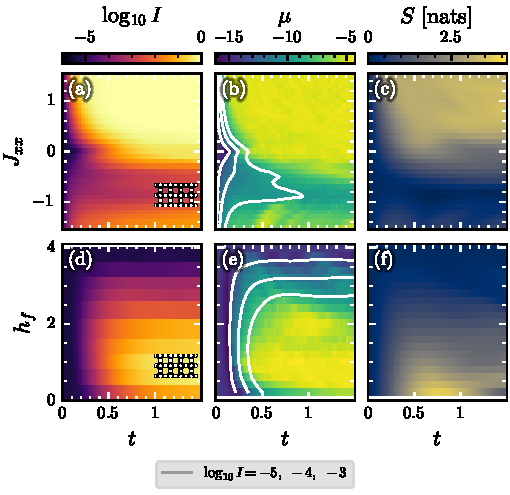
\includegraphics[width=\linewidth]{heatmaps}
  \caption{Proxies of the exact state next to the RBM infidelity, over time $t$ and control parameter. Top row:
    XY-coupling quench ($h_f=1$, control $J_{xx}$). Bottom row: field quench ($J_{xx}=0$, control $h_f$). Columns:
    cumulant proxy $\mu$ of $\log|\psi|$, phase proxy $\mu_{\mathrm{ph}}$ (white at $h_f=4=h_0$, where $\psi_0$ is
    an eigenstate and $\mu_{\mathrm{ph}}=-\infty$), half-cut entanglement entropy $S$, and $\log_{10}$ of the
    infidelity $\inff$ of the $\alpha=1$ RBM (field quench: only the 10 values of $h_f$ where TDVP was run). Lines:
    relative onset time $\tmur$ ($\mu>\mu_0+5$, white solid), end of the plateau $t_{\mathrm{dev}}$
    ($\mu>\mu_0+1.5$, white dotted), RBM failure time $\tinf$ ($\inff>10^{-3}$, cyan dashed). White insets (here and
    in later heatmaps): final Hamiltonian, initial state and the $4\times3$ cylinder (stubs: bonds across the
    periodic boundary).}
  \label{fig:edheat}
\end{figure}

\begin{figure}[t]
  \centering
  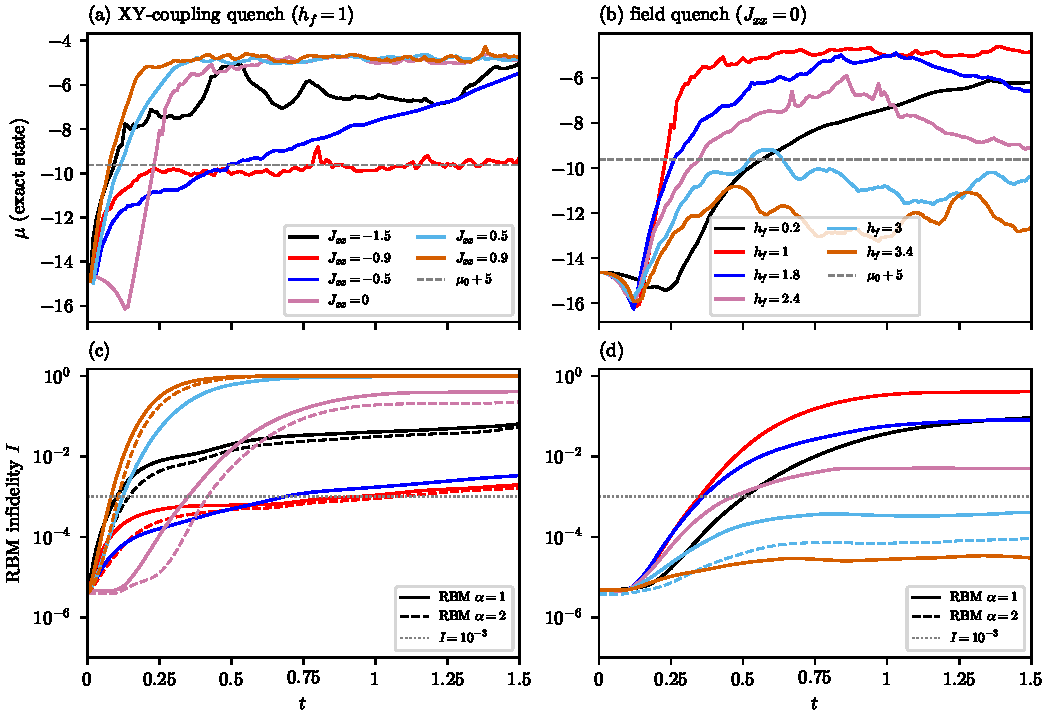
\includegraphics[width=\linewidth]{mu_inf_cuts}
  \caption{Cumulant proxy of the exact state (top) and RBM infidelity (bottom) along time, at representative control
    parameters; equal colours mark the same quench. Left: XY-coupling quench ($h_f=1$, control $J_{xx}$). Right: field
    quench ($J_{xx}=0$, control $h_f$). (a,b)~$\mu(t)$; grey dashed: threshold $\mu_0+5$ that defines the relative
    onset time $\tmur$. (c,d)~Infidelity $\inff$ of the RBM with $\alpha=1$ (solid) and $\alpha=2$ hidden units per
    spin (dashed, run at $J_{xx}\in\{-1.5,-0.9,0,0.9\}$ and $h_f=3$); grey dotted: $\inff=10^{-3}$, which defines the
    failure time $\tinf$. Both quenches start from the ground state of the 2D TFI paramagnet ($h_0=4$) on the
    $4\times3$ cylinder.}
  \label{fig:edcuts}
\end{figure}

The field quench shows a clean ``plateau then jump''; the XY-coupling quench has a $10\times$ range of onset times but
almost no plateau.

\paragraph{Field quench} (Figs.~\ref{fig:edheat}, \ref{fig:edcuts}b).
\begin{itemize}
  \item $\mu$ stays flat (or even dips slightly) up to $t_{\mathrm{dev}}\approx0.18$--$0.35$ for
    all $h_f$.
  \item For quenches deep into the ferromagnetic side ($h_f\lesssim2.4$), $\mu$ then rises to
    $\approx-5$.
  \item $\tmur$ is shortest ($0.24$) around $h_f\approx1$--$1.4$ and grows towards both $h_f\to0$
    ($0.57$) and $h_f\to h_c$ ($0.53$ at $h_f=3$).
  \item For $h_f\ge3.2$, $\mu$ never crosses threshold.
\end{itemize}

\paragraph{XY-coupling quench} (Figs.~\ref{fig:edheat}, \ref{fig:edcuts}a).
$\tmur$ runs from $0.06$ at $J_{xx}=1.5$ to $0.78$ at $J_{xx}=-0.9$. The plateau, however, is short:
\begin{itemize}
  \item $t_{\mathrm{dev}}\le0.07$ whenever $|J_{xx}|\ge0.4$, because a sudden XY coupling acts
    immediately on the $\sigma^z$ amplitudes;
  \item near the SU(2) ferromagnet ($J_{xx}\in[-0.9,-0.6]$), $\mu$ jumps quickly to $\approx-10$
    and then \emph{plateaus} there, just at the threshold;
  \item for $J_{xx}>0$, $\mu$ saturates at $\approx-5$ within $t\lesssim0.25$, while $S$ keeps
    growing to $3.5$ (out of a maximum of $4.2$).
\end{itemize}
$\tmur$ is discontinuous between $J_{xx}=-1.0$ ($0.19$) and $-0.9$ ($0.78$). The reason is that the
plateau value of $\mu$ sits at the threshold, so a small change in the plateau moves $\tmur$ by a
lot.

\begin{figure}[t]
  \centering
  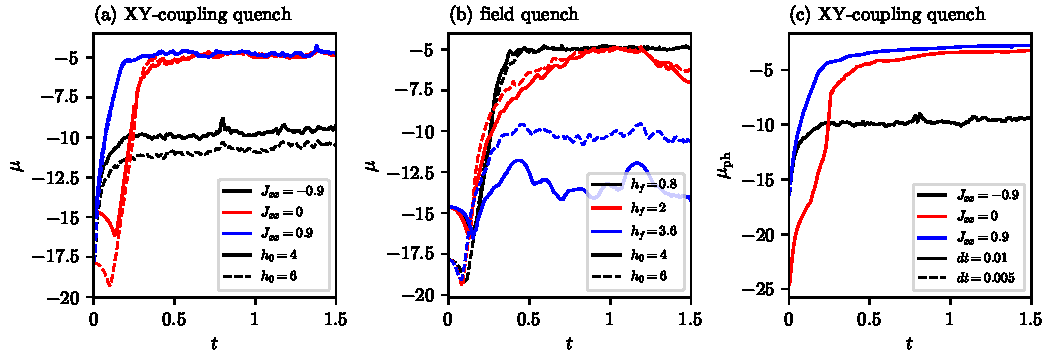
\includegraphics[width=\linewidth]{robustness}
  \caption{Robustness. (a,b)~$\mu(t)$ for initial fields $h_0=4$ (solid) and $h_0=6$ (dashed).
    (c)~$\mu_{\mathrm{ph}}$ with $dt=0.01$ (solid) and $dt=0.005$ (dashed).}
  \label{fig:robust}
\end{figure}

A scan of the full $(J_{xx},h_f)$ plane (App.~\ref{app:plane}) shows that a larger $h_f$ widens the range of onset
times but does not lengthen the plateau.

\paragraph{Robustness} (Fig.~\ref{fig:robust}). The time step is sufficient; the relative threshold is not robust to
the initial state.
\begin{itemize}
  \item \emph{Phase unwrapping.} Halving $dt$ changes $\mu$ and $\mu_{\mathrm{ph}}$ by less than
    $3\times10^{-6}$ at $J_{xx}=-0.9$ and $0$. At $J_{xx}=0.9$ the changes are $0.008$ ($\mu$) and
    $0.16$ ($\mu_{\mathrm{ph}}$), so $dt=0.01$ is sufficient.
  \item \emph{Initial field.} Raising $h_0$ to $6$ lowers $\mu_0$ from $-14.6$ to $-17.9$. The
    late-time values are nearly unchanged for hard quenches. The relative threshold
    $\mu_0+5$, however, is then crossed earlier, and in two cases at $t\approx0.2$ instead of late
    or never:
    \begin{itemize}
      \item $J_{xx}=-0.9$: $\tmur=0.07$ instead of $0.78$;
      \item $h_f=3.6$: $\tmur=0.21$ instead of never.
    \end{itemize}
    An absolute threshold ($\mu>-10$, used in Part~II) is more transferable.
\end{itemize}

\section{RBM infidelity versus the proxy}
\label{sec:rbm}

$\mu$ orders the RBM failure times in both quench families and predicts the infidelity beyond $S$; it loses resolution once
it saturates at $\approx-5$.

\begin{figure}[t]
  \centering
  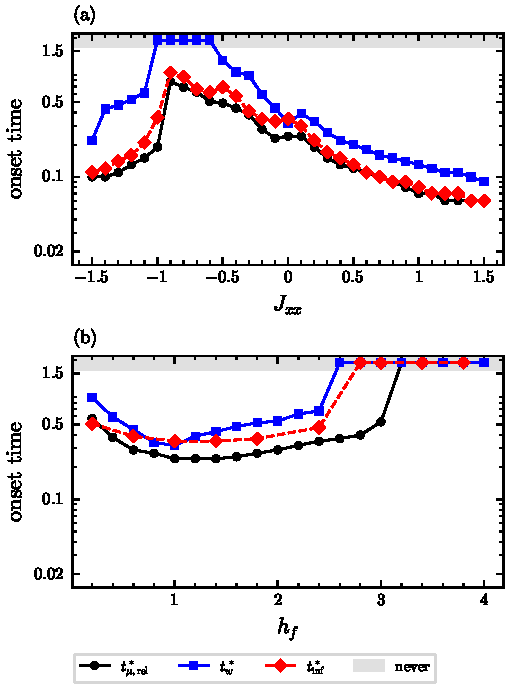
\includegraphics[width=\linewidth]{tstar_overlay}
  \caption{Onset times against the control parameter. Points in the grey band never cross their
    threshold for $t\le1.5$.}
  \label{fig:tstar}
\end{figure}

\paragraph{Onset times.}
The proxy and the RBM infidelity agree qualitatively over the whole $(t,p)$ plane
(Fig.~\ref{fig:edheat}, right column). Fig.~\ref{fig:tstar} compares the onset times quantitatively.
\begin{itemize}
  \item \emph{XY-coupling quench.} $\tmur$ and $\tinf$ follow each other almost point by point (Spearman
    $0.99$ across $J_{xx}$). This includes the sharp maximum at $J_{xx}=-0.9$ ($\tmur=0.78$,
    $\tinf=0.94$). Typically $\tinf\gtrsim\tmur$, i.e.\ $\mu$ gives a slightly early warning.
  \item \emph{Field quench.} The Spearman correlation is $0.91$.
    \begin{itemize}
      \item The two ``never'' points of $\mu$ ($h_f=3.4$ and $3.8$) end at
        $\inff=3.0\times10^{-5}$ and $5.9\times10^{-6}$.
      \item $h_f=2.8$ and $3.0$ are marginal: $\mu$ just crosses the threshold at $\tmur=0.40$ and
        $0.53$, while $\inff$ saturates just below $10^{-3}$ ($7.8\times10^{-4}$ and
        $4.0\times10^{-4}$).
    \end{itemize}
  \item \emph{Fit-free proxy.} $t^*_w$ ranks even better in the field quench (Spearman $0.98$) and worse
    in the XY-coupling quench ($0.95$). It flags the SU(2) region of the latter as never hard, while the infidelity
    saturates at $2$--$3\times10^{-3}$ there.
\end{itemize}

\begin{figure}[t]
  \centering
  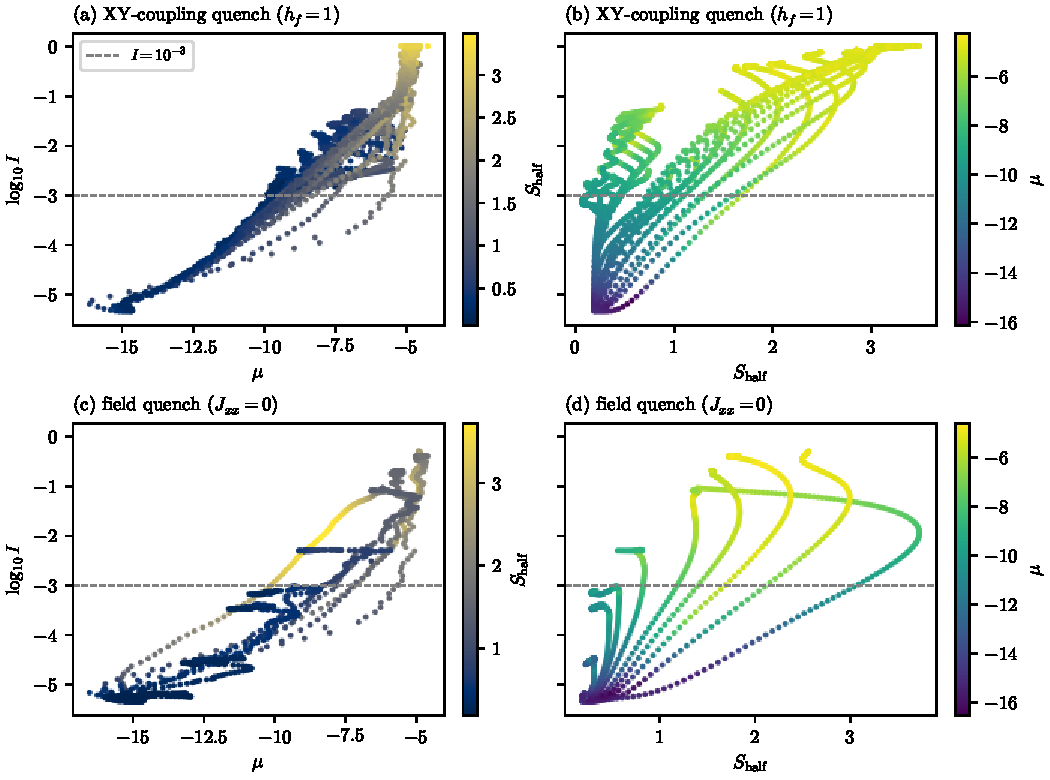
\includegraphics[width=0.95\linewidth]{scatter_mu_inf}
  \caption{Every $(t,p)$ point with $t>0$. (a,c)~$\log_{10}\inff$ against $\mu$, coloured by
    $S$. (b,d)~the same against $S$, coloured by $\mu$.}
  \label{fig:scatter}
\end{figure}


\paragraph{Pointwise relation and entanglement.}
The scatter plots (Fig.~\ref{fig:scatter}) show that $\log\inff$ is close to a monotone function
of $\mu$ for $\mu\lesssim-8$. Above that, $\mu$ saturates while the infidelity spreads over two
decades. Within that spread, a higher $S$ means a larger infidelity (panel a). This is where $\mu$
loses resolution. The $S$ panels (b,d) show the opposite structure: at fixed $S$, the infidelity
spans up to $3.5$ decades (e.g.\ $5\times10^{-6}$ to $10^{-2}$ at $S\approx0.3$ in the XY-coupling quench), ordered by $\mu$. The two
proxies are strongly correlated with each other (Spearman$(\mu,S)=0.82$ for the field quench and $0.90$ for the XY-coupling quench), so we quantify their
separate content with partial correlations (Table~\ref{tab:corr}).

\begin{table}[t]
  \centering
  \caption{Spearman correlation $\rho$ of each proxy with $\log_{10}\inff$ over all $(t,p)$ with
    $t>0$ ($n=1500$ for the field quench, $4650$ for the XY-coupling quench), and partial Spearman correlations after linearly removing
    the ranks of $S$, of $(S,t)$, or of $\mu$. Consecutive time steps are strongly autocorrelated, so the effective
    sample size is far below $n$ and no $p$-values are given.}
  \label{tab:corr}
  \footnotesize
  \setlength{\tabcolsep}{4pt}
  \begin{tabular}{llrrrr@{\hspace{2em}}llrrrr}
    \toprule
    & proxy & $\rho$ & $\rho|S$ & $\rho|S,t$ & $\rho|\mu$ & & proxy & $\rho$ & $\rho|S$ & $\rho|S,t$ & $\rho|\mu$\\
    \midrule
    field & $\mu$              & 0.96 & 0.86 & 0.86 & --    & XY & $\mu$              & 0.94 & 0.65 & 0.59 & --   \\
      & $\mu_{\mathrm{ph}}$& 0.97 & 0.92 & 0.89 & 0.62  &   & $\mu_{\mathrm{ph}}$& 0.98 & 0.88 & 0.83 & 0.82 \\
      & $w_{\mathrm{hi}}$  & 0.97 & 0.89 & 0.87 & 0.50  &   & $w_{\mathrm{hi}}$  & 0.98 & 0.86 & 0.83 & 0.80 \\
      & $S$                & 0.84 & --   & --   & 0.33  &   & $S$                & 0.91 & --   & --   & 0.49 \\
    \midrule
    \multicolumn{12}{l}{Pooled: $\rho(\mu)=0.96$, $\rho(\mu|S)=0.81$, $\rho(\mu|S,t)=0.78$;
      $\rho(S|\mu)=0.32$; $\rho(\mu_{\mathrm{ph}}|S)=0.92$; $\rho(w_{\mathrm{hi}}|S)=0.91$.}\\
    \bottomrule
  \end{tabular}
\end{table}

\paragraph{Correlation analysis.}
Table~\ref{tab:corr} gives the key test of the plan.
\begin{itemize}
  \item After removing $S$, $\mu$ keeps a large partial correlation with the infidelity:
    $0.86$ (field), $0.65$ (XY coupling), $0.81$ (pooled). This survives additionally removing $t$ ($0.78$
    pooled).
  \item The converse is much weaker. Once $\mu$ is known, $S$ adds only $0.33$ (field) and $0.49$ (XY coupling).
    So $\mu$ carries most of the information in $S$ about RBM hardness, and more besides.
  \item $\mu_{\mathrm{ph}}$ and $w_{\mathrm{hi}}$ do best (pooled $\rho|S\approx0.92$), and they
    retain $0.50$--$0.82$ even after controlling for $\mu$ (higher in the XY-coupling quench). This mainly reflects their resolution in
    the regime where $\mu$ has saturated.
  \item The auxiliary proxies $\mu_2$, $T$ and minlog add nothing beyond $\mu$ ($|\rho(\cdot|\mu)|\le0.28$). The
    near-node indicator, which drives the jump in 1D, also carries almost no information independent of $S$ in 2D
    ($\rho|S=-0.37$ for the field quench, $-0.06$ for the XY-coupling quench).
\end{itemize}

\paragraph{Larger RBM.}
Doubling the hidden units (Fig.~\ref{fig:edcuts}c,d, dashed lines) does not change the picture.
\begin{itemize}
  \item \emph{Easy and intermediate quenches} improve by a factor of $1.2$--$4.4$:
    \begin{itemize}
      \item $h_f=3$: $4.0\times10^{-4}\to9.1\times10^{-5}$;
      \item $J_{xx}=-0.9$: $2.0\times10^{-3}\to1.6\times10^{-3}$;
      \item $J_{xx}=0$: $0.41\to0.23$.
    \end{itemize}
  \item \emph{Hard quenches} are essentially unaffected: at $J_{xx}=0.9$, $\inff$ exceeds $0.9$
    at $t=0.46$ for $\alpha=1$ and at $t=0.52$ for $\alpha=2$.
\end{itemize}
In the high-$\mu$ regime, the failure is therefore not cured by modestly increasing the
expressivity.

\section{Verdict of Part I}
\label{sec:verdict1}

All three success criteria of the plan are met (Table~\ref{tab:verdict1}).

\begin{table}[h]
  \centering
  \caption{Success criteria of \texttt{PLAN\_quench\_family.md}.}
  \label{tab:verdict1}
  \small
  \begin{tabular}{p{6.6cm}p{6.6cm}c}
    \toprule
    criterion & result & met\\
    \midrule
    $\tmur(p)$ and $\tinf(p)$ agree in ordering, Spearman $\ge0.8$ & field: $0.91$; XY coupling: $0.99$ & yes\\
    ``Never hard'' points in $\mu$ have $\inff<10^{-3}$ at $t=1.5$ & field, $h_f=3.4$: $3.0\times10^{-5}$; $h_f=3.8$: $5.9\times10^{-6}$ (XY coupling has no never points) & yes\\
    $\mu$ predicts beyond $S$ & partial $\rho(\mu|S)=0.81$ pooled (field $0.86$, XY coupling $0.65$) vs $\rho(S|\mu)=0.32$ & yes\\
    \bottomrule
  \end{tabular}
\end{table}

\paragraph{Where $\mu$ works.}
\begin{itemize}
  \item It predicts the RBM failure time $\tinf$ across a $10\times$ range of onset times, and it
    usually fires slightly before the infidelity crosses $10^{-3}$.
  \item It correctly identifies the slow region around the SU(2) ferromagnet. There, $\mu$ and
    $\inff$ both saturate at a low plateau ($\mu\approx-9.5$, $\inff\approx2\times10^{-3}$).
  \item It correctly identifies the paramagnetic side of the field quench as easy.
  \item It carries information on RBM hardness that the entanglement entropy does not.
\end{itemize}

\paragraph{Where $\mu$ fails or is fragile.}
\begin{enumerate}
  \item \emph{Saturation.} $\mu$ caps at $\approx-5$ once the spectrum is dense, so it cannot rank
    hard quenches against each other. Over the saturated region, $\inff$ ranges from $0.06$ to
    $1$. $S$, $\mu_{\mathrm{ph}}$ and $w_{\mathrm{hi}}$ keep resolving it.
  \item \emph{Strong ferromagnetic XY ($J_{xx}=-1.5$).} $\mu$ reaches $-5$ (as ``hard'' as the TFI
    quench at $J_{xx}=0$), but the infidelity only reaches $0.065$, against $0.41$ at $J_{xx}=0$.
    The low entanglement ($S=0.87$) is the better guide here. This is the decoupling point
    flagged in the plan, and at it $\mu$ \emph{overestimates} the difficulty.
  \item \emph{No plateau in the XY-coupling quench.} With $|J_{xx}|\ge0.4$, $\mu$ starts moving after
    $t_{\mathrm{dev}}=0.02$--$0.07$, while $\inff$ first exceeds $10^{-4}$ only at $t=0.04$--$0.17$,
    i.e.\ $2$--$3\times$ later. Only the field quench has a real
    ``flat then jump'' plateau.
  \item \emph{Threshold dependence.} $\tmur$ is defined relative to $\mu_0$, so it is sensitive to the
    initial state (Fig.~\ref{fig:robust}). It is also discontinuous where $\mu$ plateaus close to
    threshold ($J_{xx}=-1.0$ versus $-0.9$).
\end{enumerate}

\paragraph{Recommendation.}
\begin{itemize}
  \item Use the XY-coupling quench ($h_f=1$, control $J_{xx}$) as the primary family: it has the widest and most
    faithfully tracked range of $\tinf$.
  \item Keep the field quench as the reference for the clean plateau-then-jump and ``never hard''
    behaviour.
  \item For a quantitative hardness predictor beyond the onset time, report $\mu_{\mathrm{ph}}$ or
    the fit-free $w_{\mathrm{hi}}$ alongside $\mu$. They do not saturate as early and have the
    highest partial correlations.
  \item Replace the relative threshold by an absolute one (e.g.\ $\mu>-10$) before comparing
    different initial states.
\end{itemize}

\paragraph{Limitations.}
\begin{itemize}
  \item \emph{System size.} With 12 sites and a 3-site open direction, DQPT-like features are
    smeared. $h_c(4\times3)$ is not the bulk $3.04$, and every $t^*$ is a crossover time.
  \item \emph{Error sources.} The TDVP infidelity mixes expressivity with integration and
    QGT-inversion error. The solver settings were kept fixed across $p$, but they were not varied.
  \item \emph{Correlation statistics.} The correlations (here and in Part~II) pool strongly autocorrelated time
    series, so the numbers are descriptive and not significance tests.
  \item \emph{Threshold choices.} The thresholds $\mu_0+5$, $1\%$ and $10^{-3}$ follow the plan and
    were not tuned.
\end{itemize}

\FloatBarrier
\part{Rydberg and related quenches}

\section{Targets and approach}
\label{sec:ryd}

Part~II (\texttt{PLAN\_rydberg\_quench.md}) asks whether there are quenches in which the entanglement grows fast, so
that the state becomes expensive for MPS, while the RBM+TDVP infidelity stays small. We call this an \emph{RBM
advantage} and distinguish two targets:
\begin{itemize}
  \item \emph{Near-classical RBM advantage}: $H_f$ is close to diagonal in $\sigma^z$ ($\eta\lesssim0.1$). The
    amplitudes barely move and the phase is generated by two-body Ising terms, which an RBM with enough hidden units,
    or a Jastrow factor, can encode exactly, while the half-cut entanglement of such phase states is volume-law.
  \item \emph{Quantum RBM advantage} (``gold'' in the plan): the same with a genuinely non-classical $H_f$
    ($\eta\ge0.3$), and with $\mu$ and $\mu_{\mathrm{ph}}$ staying below $-10$ until $t_S$.
\end{itemize}

\paragraph{Approach.}
\begin{itemize}
  \item \emph{Screen.} 37 quench families (976 parameter points) realised in Rydberg, dipolar and trapped-ion
    experiments, NQS benchmarks and theory, evolved exactly on 12--16 sites, with the proxies and the entanglement at
    every time step (Apps.~\ref{app:rydsetup}, \ref{app:screen}).
  \item \emph{RBM runs.} Six Tier-1 families followed with 159 full-sum RBM/Jastrow+TDVP runs (App.~\ref{app:stage3}).
  \item \emph{Main text.} Two families carry the conclusions: R1, the best near-classical case, and G4, a standard NQS
    benchmark and the closest approach to a quantum RBM advantage.
\end{itemize}

\paragraph{The two highlighted families.} Both run on the $4\times3$ cylinder of Part~I (R1 also on the $4\times4$
torus). With $n_i=(1-Z_i)/2$ and $V_{ij}=V_{nn}(a/r_{ij})^6$, the Rydberg Hamiltonian is
\begin{equation}
  H_{\mathrm{Ryd}}=\frac\Omega2\sum_iX_i-\Delta\sum_in_i+\sum_{i<j}V_{ij}n_in_j ,
\end{equation}
with Rabi frequency $\Omega$, detuning $\Delta$, and time in units of $1/V_{nn}$.
\begin{itemize}
  \item \textbf{R1, 2D Rydberg Ising quench}~\cite{Lienhard18,GuardadoSanchez18}: $H_{\mathrm{Ryd}}$ with $\Delta=0$
    from $|{+}x\rangle$, control parameter $\Omega/V_{nn}$ from $0$ (classical) to $1$ (13 values), $t\le3/\Omega$.
    Small $\Omega$ is near-classical ($\eta=0.005$ at $\Omega/V_{nn}=0.01$, $0.45$ at $1$).
  \item \textbf{G4, 2D TFI benchmark}~\cite{SchmittHeyl20}: Schmitt and Heyl simulated 2D TFI quenches with
    convolutional NQS at $h_f=h_c/10$, $h_c$ and $2h_c$ ($h_c=3.04438$). We use $H=-\sum_{i<j}(a/r_{ij})^6Z_iZ_j-h_f\sum_iX_i$
    from the paramagnetic ground state of Part~I ($h=4$), with 13 values of $h_f$ including these three, $t\le10$. It
    is non-classical for $h_f\gtrsim0.6$ ($\eta=0.42$--$0.98$).
\end{itemize}

\paragraph{RBM runs.} An $\alpha=1$ RBM over the full grid; at three points per family $\alpha=2$, $\alpha=4$ and a
pure Jastrow factor; RBM$\times$Jastrow at R1 $\Omega/V_{nn}=0.05$; and an $\alpha=1$ RBM on the $4\times4$ torus
($N=16$) for R1. TDVP sums over all $2^N$ configurations, so there is no Monte Carlo noise. Product starts are exact
through the visible biases (initial $\inff\approx10^{-9}$); the ground-state start of G4 is fitted by SR (initial
$\inff\approx3\times10^{-6}$). Runs stop once $\inff\ge0.5$. Solver settings: App.~\ref{app:num}.

\section{Screen: near-classical windows, no quantum RBM advantage}
\label{sec:screen}

\begin{figure}[t]
  \centering
  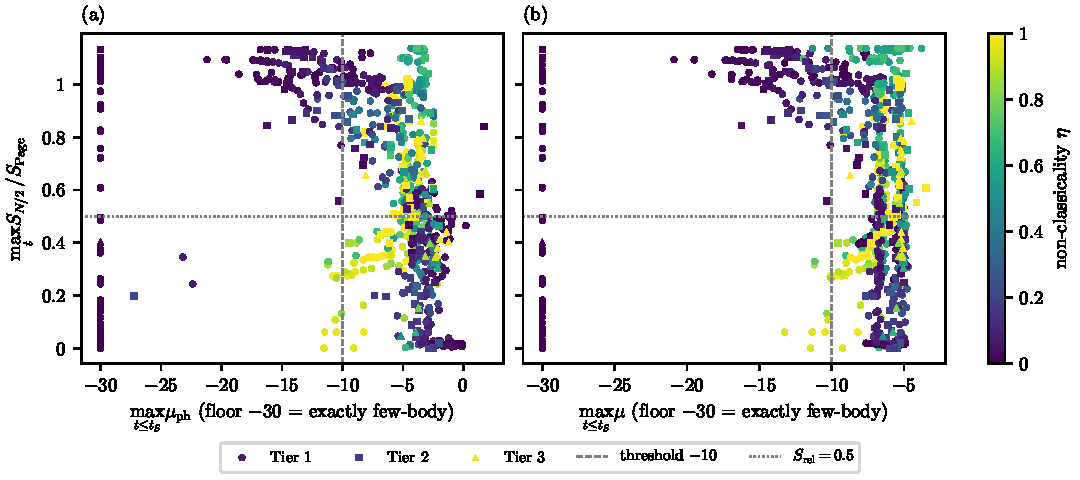
\includegraphics[width=\linewidth]{map}
  \caption{Every screened point (976 points, 37 families, 81 cluster/initial-state combinations), placed by its
    largest half-cut entropy relative to Page (vertical) and by the largest value of (a)~$\mu_{\mathrm{ph}}$, (b)~$\mu$
    reached up to $t_S$ (or over the whole run if $S_{\mathrm{rel}}$ never reaches $0.5$). Colour: non-classicality
    $\eta$. The yellow upper-left region (MPS-hard, proxies below $-10$) is where a quantum RBM advantage would sit; it
    is empty. The points at the floor $-30$ are exactly classical.}
  \label{fig:map}
\end{figure}

The screen finds many near-classical windows and no candidate for a quantum RBM advantage (Fig.~\ref{fig:map}).
\begin{itemize}
  \item \emph{No quantum candidate.} Of the 619 points that become MPS-hard, 356 have $\eta\ge0.3$; for none of them
    do both proxies stay below $-10$ until $t_S$. The largest proxy window among them is $1.0$ (median $0.25$): in
    non-classical quenches the proxies fire no later than the entanglement saturates, usually much earlier.
  \item \emph{Near-classical windows are common.} Of the 201 MPS-hard points with $\eta\le0.1$, 53\% have a proxy
    window $\ge2$. The strongest is R1 (up to 38 at $\Omega/V_{nn}=0.01$).
\end{itemize}
Per-family results of the screen are in App.~\ref{app:screen}.

\section{R1: a near-classical RBM advantage}
\label{sec:r1}

\begin{figure}[t]
  \centering
  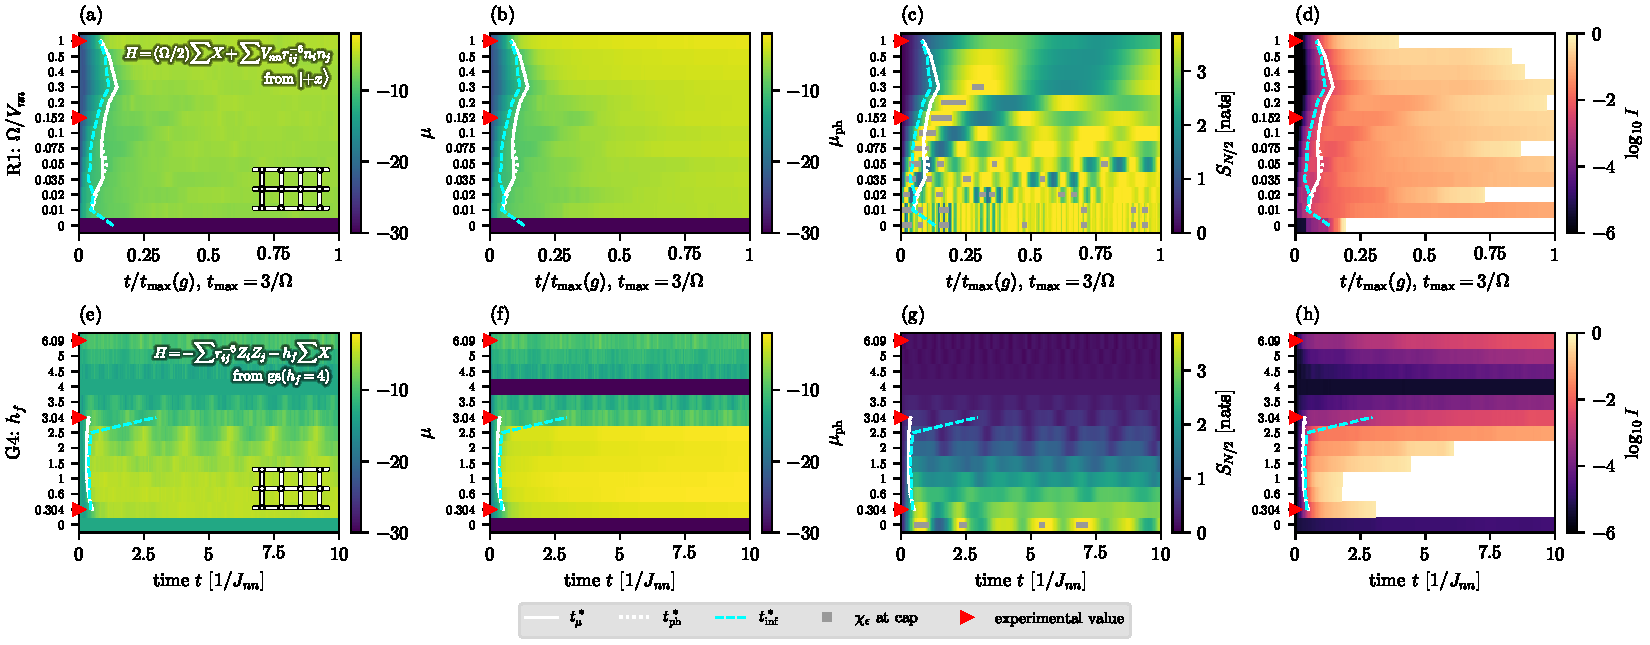
\includegraphics[width=\linewidth]{main_rows_hl}
  \caption{R1 (top) and G4 (bottom) over control parameter $g$ (vertical, one strip per grid point) and time.
    Insets as in Fig.~\ref{fig:edheat}. Columns: $\mu$, $\mu_{\mathrm{ph}}$, half-cut entropy $S$ (grey squares:
    $\chi_\varepsilon$ at its cap), and $\log_{10}\inff$ for the $\alpha=1$ RBM (white: run stopped at $\inff\ge0.5$).
    Lines: $\tmu$ (white solid), $\tph$ (white dotted), $\tinf$ (cyan dashed). Red triangles: experimental or benchmark
    values of $g$. R1 is plotted against $t/t_{\max}(g)$, $t_{\max}=\min(300,\max(10,3/\Omega))$.}
  \label{fig:main-rows-hl}
\end{figure}

\begin{figure}[t]
  \centering
  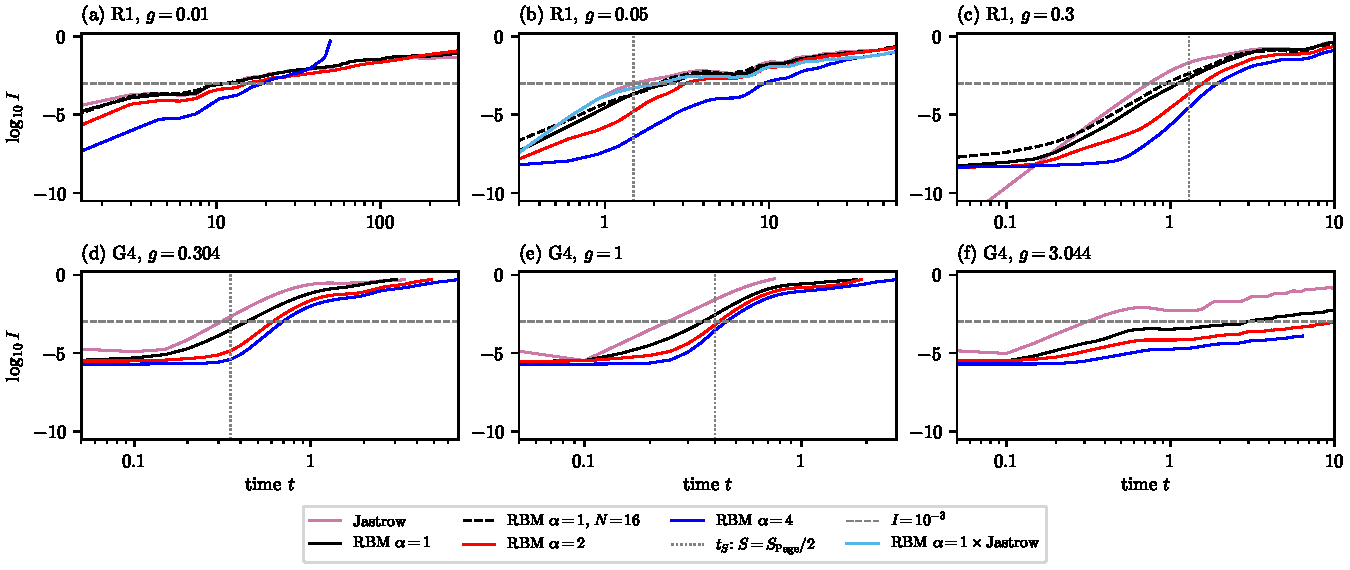
\includegraphics[width=\linewidth]{ansatz_hl}
  \caption{$\log_{10}\inff(t)$ per ansatz at three points of R1 (top) and G4 (bottom), logarithmic time axis. Dashed
    black: $\alpha=1$ RBM on the $4\times4$ torus ($N=16$). Dotted vertical: $t_S$ (the state becomes MPS-hard at
    $N=12$); dashed horizontal: $\inff=10^{-3}$. Time in units of $1/V_{nn}$ (R1) and $1/J_{nn}$ (G4).}
  \label{fig:ansatz-hl}
\end{figure}

In the weakly driven 2D Rydberg Ising quench the RBM follows a volume-law state for up to $12\,t_S$
(Figs.~\ref{fig:main-rows-hl}, \ref{fig:ansatz-hl}a--c).
\begin{itemize}
  \item \emph{RBM window.} At $\Omega/V_{nn}=0.01$ the infidelity stays below $10^{-3}$ up to $t=12$ ($\alpha=1$,
    Jastrow), $15$ ($\alpha=2$) and $18$ ($\alpha=4$), while $S_{\mathrm{rel}}\ge0.5$ from $t_S=1.5$ on and reaches
    $1.13$: an RBM window of $8$--$12$. At $\Omega/V_{nn}=0.05$ the RBM is accurate up to $t=2.4$ ($\alpha=1$), $3.0$
    ($\alpha=2$) and $9.3$ ($\alpha=4$), an RBM window of $1.6$--$6$. For $\alpha=1$ the window closes at
    $\Omega/V_{nn}\approx0.15$.
  \item \emph{More hidden units help, a Jastrow factor does not.} Going from $\alpha=1$ to 4 delays $\tinf$ by
    $1.4$--$3.6\times$ and lowers the early infidelity by 1--3 decades. The Jastrow factor alone is no better than
    $\alpha=1$ ($\Omega/V_{nn}=0.01$: $\tinf=10.5$ vs $13.5$), and RBM$\times$Jastrow is no better than the RBM alone
    ($0.05$: $2.4$ vs $2.7$). The error therefore comes from the weak drive, not from the Ising phase.
  \item \emph{Larger cluster.} At $N=16$, $\tinf$ is equal or $10$--$20\%$ shorter ($0.01$: $13.5\to12$; $0.05$:
    $2.7\to2.4$; $0.3$: $1.15\to0.95$), while $t_S$ is unchanged and the proxy onsets move later ($\tmu$ at $0.05$:
    $5.4\to9.6$). The entanglement per boundary bond is the same for both sizes (App.~\ref{app:stage3},
    Fig.~\ref{fig:scaling}), so the window survives the step in $N$ but does not grow.
  \item \emph{Proxies rank well but fire late.} $\mu_{\mathrm{ph}}$ predicts the infidelity (Spearman $0.92$, also
    $0.92$ at fixed $S$; $\mu$: $0.85$; $S$ alone: $0.14$), and $\tprox$ orders $\tinf$ perfectly across $\Omega$
    ($\rho=1.00$). But the RBM fails before the proxies at all 12 points (median $\tinf/\tprox=0.77$), so the proxy
    window overstates the RBM window by $\approx25\%$.
  \item \emph{The window shrinks with $\Omega$.} $\tmu\Omega\approx0.15$--$0.75$ for $\Omega/V_{nn}\le0.2$, while
    $t_S\approx1.0$--$1.5$ is set by the Ising couplings; the proxy window closes at $\Omega/V_{nn}\approx0.1$--$0.2$.
\end{itemize}
The same near-classical behaviour appears in Rydberg-dressed interferometry (R6, App.~\ref{app:stage3}), at the
experimental soft-core radius with an RBM window of $1.5$--$4.5$.

\section{G4: no quantum RBM advantage}
\label{sec:g4}

In the 2D TFI benchmark, proxy onset, RBM failure and entanglement saturation coincide; there is no window
(Figs.~\ref{fig:main-rows-hl}, \ref{fig:ansatz-hl}d--f).
\begin{itemize}
  \item \emph{The RBM fails at $t_S$.} For $0<h_f\le2.5$ the $\alpha=1$ RBM crosses $10^{-3}$ at $t=0.35$--$0.45$.
    Where the state becomes MPS-hard ($h_f\le1$, $t_S=0.30$--$0.40$), this is at or one save step after $t_S$; for
    $h_f\ge1.5$ the entropy stays below half the Page value. Close to the initial field ($h_f\ge3$) the quench is
    easy ($\tinf=2.95$ at $h_c$, never for $h_f=3.5$--$5$).
  \item \emph{More hidden units barely help.} $\alpha=4$ delays $\tinf$ by at most $1.6\times$ ($h_f=0.304$:
    $0.45\to0.70$; $h_f=1$: $0.40\to0.45$).
  \item \emph{Closest approach.} $h_f=0.6$ ($\eta=0.42$) and $h_f=1$ ($\eta=0.61$) are the only screened points with
    $\eta\ge0.3$ where $S_{\mathrm{rel}}\ge0.5$ and $\inff<10^{-3}$ hold at the same time, each only at the single save
    time $t=t_S$ ($h_f=0.6$: $t_S=0.35$, with $\alpha=1$; $h_f=1$: $t_S=0.40$, with $\alpha=2$ and $4$). The proxies
    have already fired at $0.30$--$0.35$, and $\inff$ crosses $10^{-3}$ one step later. At $N=12$,
    $S_{\mathrm{rel}}=0.5$ means $S\approx1.8$ nats, so this is not a meaningful MPS-hard window. At $h_f=h_c/10$
    ($\eta=0.23$, below the non-classical threshold) the RBM window is $1.9$ ($\alpha=4$).
  \item \emph{The proxies work.} $\mu_{\mathrm{ph}}$ predicts the infidelity best (Spearman $0.94$, $0.93$ at fixed
    $S$; $\mu$: $0.91$; $S$ alone: $0.29$), and fires first (median $\tinf/\tprox=1.33$; the RBM fails first at only
    1 of 8 points). The onset ordering across $h_f$ is $\rho=0.64$ ($\tmu$) and $0.72$ ($\tph$).
  \item \emph{Mechanism.} The same holds in every non-classical family (D3, R4; App.~\ref{app:stage3}): the proxies
    fire no later than $t_S$ and the RBM fails at about the same time ($\tinf\approx1.3\,\tprox$). On 12--16 sites,
    fast entanglement growth from a non-classical $H_f$ comes with amplitude dynamics that fill the cluster spectrum
    of $\log|\psi|$, and that is what the RBM cannot follow (interpretation, not tested separately). The Clifford
    kicked Ising circuit, a natural candidate, fails for a different reason (App.~\ref{app:stage3}).
\end{itemize}

\section{Verdict of Part II}
\label{sec:verdict2}

Three of the four success criteria are met; the quantum RBM advantage is not (Table~\ref{tab:verdict2}).

\begin{table}[h]
  \centering
  \caption{Success criteria of \texttt{PLAN\_rydberg\_quench.md}.}
  \label{tab:verdict2}
  \small
  \begin{tabular}{p{5.2cm}p{8.2cm}c}
    \toprule
    criterion & result & met\\
    \midrule
    Near-classical RBM advantage: $S_{\mathrm{rel}}\ge0.5$ with $\inff<10^{-3}$ ($\alpha\le2$ or RBM$\times$Jastrow)
      & R1 $\Omega/V_{nn}=0.01$: $t_S=1.5$, $\inff<10^{-3}$ up to $t=12$ ($\alpha=1$), $15$ ($\alpha=2$); R6: up to
        $2.4$--$3.6$ ($\alpha\le2$, $t_S=1.2$--$1.5$); also at $N=16$ & yes\\
    Quantum RBM advantage: the same with $\eta\ge0.3$ and $\mu,\mu_{\mathrm{ph}}<-10$
      & none; closest: G4 $h_f=1$, one save step at $t_S$ with proxies already above $-10$ & no\\
    Relevance: headline from Tier~1 & R1~\cite{Lienhard18,GuardadoSanchez18} and R6~\cite{Zeiher16,Zeiher17} are Tier~1 & yes\\
    Proxy validity: Spearman $\ge0.8$ and partial $\ge0.5$ in $\ge2$ new families
      & $\mu_{\mathrm{ph}}$: R1 $0.92/0.92$, G4 $0.94/0.93$, D3 $0.93/0.87$, I1 $0.82/0.80$; fails in R4 & yes\\
    \bottomrule
  \end{tabular}
\end{table}

\begin{itemize}
  \item Near-classical quenches with a weak drive ($\Omega/V_{nn}\lesssim0.05$) are the regime where an RBM follows a
    volume-law state for several times $t_S$; a larger hidden-unit density helps, the exact Jastrow factor does not.
  \item The proxy window is the right screen for this regime (it selected R1, R6, I1), but it overstates the RBM
    window: in R1 the RBM fails at $\approx0.8\,\tprox$.
  \item In non-classical quenches the proxies, the RBM failure and the entanglement saturation coincide within a
    factor $\approx1.3$ on 12--16 sites; we found no counterexample.
\end{itemize}

\paragraph{Limitations.}
\begin{itemize}
  \item \emph{Cluster size.} ``MPS-hard'' means $S_{\mathrm{rel}}\ge0.5$ at $N=12$--$16$, i.e.\
    $S\gtrsim1.8$--$2.5$ nats and $\chi_\varepsilon\le64$--$256$. The step $N=12\to16$ leaves the entropy per boundary
    bond unchanged (Fig.~\ref{fig:scaling}); extrapolating it to a 10-site cut gives $S\gtrsim6.8$ nats,
    $\chi\gtrsim900$, which is a rough lower bound (not sure). The $N=16$ RBMs ran only to $t=15$ and at two families.
  \item \emph{Phase proxy.} The time-unwrapped phase is not reduced modulo $2\pi$, so $\mu_{\mathrm{ph}}$
    flags stabilizer states (S3) as dense. Near nodes ($\mathrm{minlog}\approx-70$, C2/R5) it changes by up to $6$
    under $dt/2$; $\tph$ moved in one of 48 checks.
  \item \emph{TDVP.} The solver settings (App.~\ref{app:num}) were not varied. The $\Omega=0$ runs show that TDVP
    error, not expressivity, can dominate (App.~\ref{app:stage3}). Zero initial hidden biases freeze the RBM for odd
    three-body terms (I5). Four $\alpha=4$ runs stopped at the 6\,h limit.
\end{itemize}

\FloatBarrier
\appendix

\section{Calibration: 1D TFI chain}
\label{app:cal}

\begin{figure}[h]
  \centering
  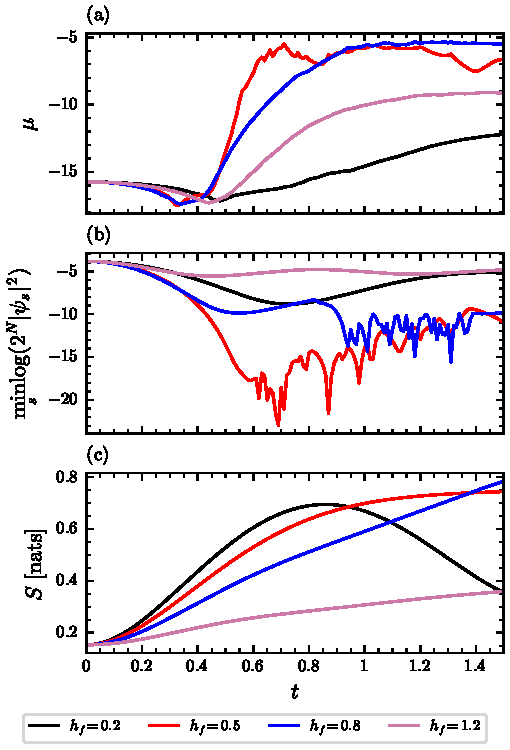
\includegraphics[width=\linewidth]{cal1d}
  \caption{1D TFI chain, $L=12$ (open boundaries), quench from the ground state at $h=1.5$ to
    $h_f$, analysed with the final code. (a)~$\mu(t)$, (b)~near-node indicator, (c)~half-chain
    entanglement.}
  \label{fig:cal}
\end{figure}

The final code reproduces the calibration of the original 1D study (Fig.~\ref{fig:cal}): the jump in $\mu$ is driven
by amplitude zeros, not by entanglement. For $h_f=0.5$:
\begin{itemize}
  \item $\mu$ stays at $-16$ to $-17$ up to $t\approx0.45$ and then jumps to $\approx-6$
    ($\tmur=0.54$);
  \item the jump coincides with a near-node of $\psi$: $\mathrm{minlog}$ reaches $-22.9$ at $t=0.69$;
  \item the entanglement stays low throughout ($S<0.8$).
\end{itemize}
The 1D picture is not purely ``onset if and only if the quench crosses $h_c=1$'', however:
\begin{itemize}
  \item $h_f=1.2$ does not cross $h_c$, yet $\mu$ drifts up to $-9$;
  \item $h_f=0.2$ does cross $h_c$, yet it stays below threshold until $t=1.5$.
\end{itemize}

\section{The $(J_{xx},h_f)$ plane}
\label{app:plane}

\begin{figure}[t]
  \centering
  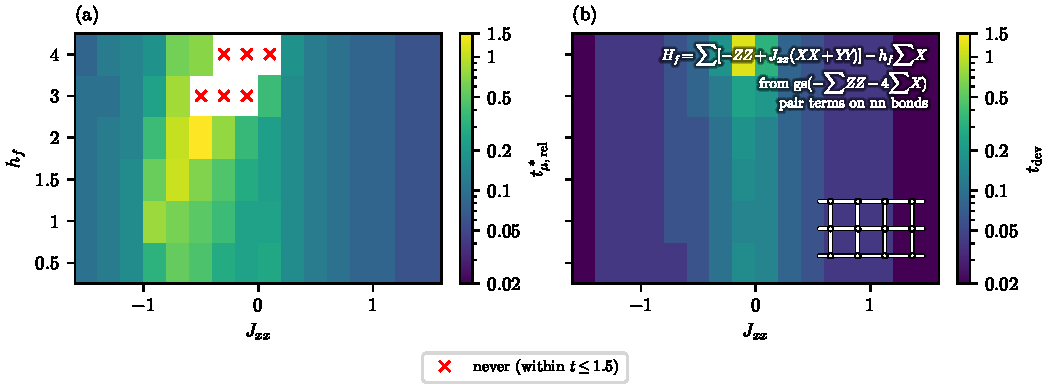
\includegraphics[width=\linewidth]{plane_tstar}
  \caption{XY-coupling quench generalised to the $(J_{xx},h_f)$ plane ($16\times6$ points, $dt=0.02$). Insets as in
    Fig.~\ref{fig:edheat}. (a)~onset time $\tmur$. (b)~plateau length $t_{\mathrm{dev}}$. Red crosses: $\mu$ never
    crosses the threshold for $t\le1.5$.}
  \label{fig:plane}
\end{figure}

The plane scan (Fig.~\ref{fig:plane}) confirms the expectation of the plan: a larger $h_f$ widens the range of onset
times but does not lengthen the plateau.
\begin{itemize}
  \item larger $h_f$ opens a ``never hard'' window at $J_{xx}\in[-0.5,0.1]$ for $h_f\ge3$;
  \item the longest finite onsets lie on the ferromagnetic side: $\tmur\approx1.0$--$1.5$ at
    $h_f=1.5$--$2$ and $J_{xx}\approx-0.7$ to $-0.5$;
  \item the plateau length $t_{\mathrm{dev}}$ stays short ($\lesssim0.15$) almost everywhere. The
    exception is the column $J_{xx}\approx-0.1$, which is close to the field quench, at large field:
    $t_{\mathrm{dev}}=0.24$ at $h_f=3$ and $1.2$ at $h_f=4$.
\end{itemize}

\FloatBarrier
\section{Part II: setup details}
\label{app:rydsetup}

\paragraph{Families.} The 37 families (Table~\ref{tab:families}) were realised in experiments, serve as benchmarks,
or are prominent in theory, sorted into three tiers: Tier~1 (realised in an experiment or an established numerical
benchmark), Tier~2 (natural variations of Tier-1 set-ups or proposals) and Tier~3 (methodological controls). Each
family has one control parameter $g$ on a grid of 6--17 values that contains the experimental values
(\texttt{rydberg/data/exp\_params.csv}). Rydberg ground state: $|{\downarrow}\rangle\equiv|g\rangle$.

\paragraph{Hamiltonian parameters.}
$\Omega$: Rabi frequency, $\Delta$: detuning, $V_{nn}$: nearest-neighbour van der Waals interaction ($V(r)=V_{nn}(a/r)^6$),
$R_b=(V_{nn}/\Omega)^{1/6}a$: blockade radius, $R_c$: soft-core radius of Rydberg dressing, $\kappa$ in $1/r^\kappa$:
interaction range of trapped-ion Ising models, $J_z/J_{xy}$: XXZ anisotropy, $\Theta$: tilt of the quantisation axis
of dipolar XY, $\theta$: tilt angle of a product initial state from $|{\uparrow}\rangle$, $h$: longitudinal field,
$\varepsilon$: small perturbation strength, $J,b$: Ising and kick angles of the kicked Ising circuit.


\paragraph{Clusters.} $N=12$ or $16$: chains (open), rings, the $4\times3$ cylinder of Part~I (\texttt{sq4x3}), the
$4\times4$ torus (\texttt{sq4x4}), $4\times3$ and $4\times4$ triangular tori, a $2\times2$-cell kagome torus
(\texttt{kag12}), a 12-site ruby strip (bond midpoints of four corner-sharing kagome triangles, open), a 12-qubit
toric code on a $2\times3$ torus, and a 12-site honeycomb torus. Long-range couplings use minimum-image distances.

\paragraph{Initial states.} Product states $|{+}x\rangle$, $|\theta\rangle$ (all spins tilted by $\theta$ from
$|{\uparrow}\rangle$; $\theta=\pi/4$ unless $\theta$ is the control parameter), $|\mathbb Z_2,\theta\rangle$ (Néel
tilted by $\theta$), $|g\rangle$ tilted by $0.1$--$0.2$ (Rydberg-native starts, tilted off the blockade zeros), and
ground states of a pre-quench Hamiltonian. The tilts keep $\log|\psi|$ finite.

\paragraph{Exact evolution.} Sparse Krylov evolution on 201 save times (21 for Floquet circuits, one per period),
with the phase unwrapped along time (App.~\ref{app:num}). Halving $dt$ at three points of every Tier-1 family (48 runs)
changes $\psi$, $S$ and $\mu$ by less than $10^{-9}$. $\mu_{\mathrm{ph}}$ changes by up to $6$ in two driven chains
(C2, R5) where $|\psi|$ comes within $e^{-70}$ of a node, but $\tph$ moves in only one of 48 checks, by one save step
(C2: $6.0\to7.5$).

\paragraph{Triage.} For every $(g,t)$ we record the quantities of Sec.~\ref{sec:defs}. A point is
\emph{MPS-hard (at this size)} from $t_S$ on. The plan's classes,
evaluated up to $t_{\max}$, are: (i)~onset ($\mu$ crosses $-10$ after a low plateau), (ii)~near-classical
($\eta\le0.1$, $S_{\mathrm{rel}}\ge0.5$, $\mu_{\mathrm{ph}}<-10$ throughout), (iii)~quantum ($\eta\ge0.3$,
$S_{\mathrm{rel}}\ge0.5$, $\mu,\mu_{\mathrm{ph}}<-10$ throughout), (iv)~boring. Because every non-classical run
eventually saturates the proxies on 12--16 sites, we also use a \emph{window} version: a point is near-classical
(quantum) if its proxy window is at least two, $\tprox/t_S\ge2$.

\paragraph{Deviations from the plan.}
\begin{itemize}
  \item Tier changes: I3 (no longitudinal field in the ion experiment~\cite{Tan21}), D6 (the experiment is a 3D
    gas~\cite{Signoles21}) and R7 (no extractable parameters) moved to Tier~2; S8 (optional) was skipped. A new
    Tier-1 axis S3b follows the IBM circuit~\cite{Kim23} ($J=\pi/4$, $h=0$, kick $b=\theta_h/2$) on a 12-site ring
    (one heavy hexagon), a chain and the cylinder.
  \item R5 uses the experimental $V_{nn}/\Omega=12$~\cite{Bernien17} instead of $30$; C2's control parameter is
    $\omega_m/\Omega$~\cite{Bluvstein21}; D4's is the staggered field $\delta$ with a balanced $\pm1$ pattern~\cite{Bintz24};
    G3 starts from the ground state of the XY ferromagnet with a small transverse field, which removes the $U(1)$
    zeros; I3 starts at $\theta=0.1$.
  \item Tier-2 and Tier-3 families run on 12-site clusters only; disorder (R7, R8, D6) uses one realisation.
  \item Stage-2/3 RBMs run at $N=12$; for families screened only at $N=16$, the $4\times3$ cylinder was added to the
    screen.
  \item Grids have 13--17 instead of 15--21 points; the window classification is an addition to the plan's strict
    classes; the RBM budget (159 runs) exceeds the plan's 30 Stage-2 probes because Stage~3 used the full grids.
\end{itemize}

\section{Part II: screen of all families}
\label{app:screen}

\paragraph{Other Stage-3 families.}
\begin{itemize}
  \item \emph{R0/R6, Rydberg-dressed Ising interferometry}~\cite{Zeiher16,Zeiher17,Borish20}: $|{+}x\rangle$ evolves
    under the soft-core interaction $U_0/(1+(r/R_c)^6)$ (experiment: $R_c/a=2.02$). Without a drive (R0) the phase is
    exactly two-body, so $\mu=\mu_{\mathrm{ph}}=-\infty$ and a Jastrow factor is exact, while $S$ can reach the Page
    value. R6 adds a weak drive $\Omega=0.05$.
  \item \emph{R4, Rydberg arrays at fixed blockade radius}~\cite{Ebadi21,Samajdar20,Semeghini21,Verresen21}: quench at
    $\Delta=0$, $R_b/a$ across the experimental values $1.15$ (checkerboard), $1.53$ (ruby) and $2.4$.
  \item \emph{D3, Floquet-engineered dipolar XXZ}~\cite{Scholl22,Geier21}: from $|{+}x\rangle$, $J_z/J_{xy}$ runs from
    Ising-like via XY to Heisenberg ($J_z/J_{xy}=1$, where $|{+}x\rangle$ is an eigenstate); strongly non-classical
    ($\eta\approx0.8$).
  \item \emph{I1, trapped-ion long-range Ising}~\cite{Richerme14,Jurcevic14,Jurcevic17,Zhang17}: ion chains realise
    $\sum_{ij}J_0|i-j|^{-\kappa}X_iX_j+B\sum Z_i$ with $\kappa\approx0.6$--$1.2$, and dynamical quantum phase
    transitions, the 1D mechanism behind the jump of $\mu$~\cite{Heyl13}, were observed there. Here: $\sum
    r^{-\kappa}ZZ$ with a weak transverse field ($0.1$) from $|{+}x\rangle$; near-classical, range set by $\kappa$.
  \item \emph{S3/S3b, kicked Ising near Clifford points}~\cite{Kim23,Tindall24,Begusic24,BKP18,BKP19}: at $J=b=\pi/4$
    the circuit is dual-unitary with maximal entanglement growth, yet from $|{+}x\rangle$ at $h=0$ it produces
    stabilizer states (flat $\log|\psi|$, phase quadratic mod $2\pi$): the most natural quantum candidate.
\end{itemize}

\paragraph{Screen results per family} (Fig.~\ref{fig:map}).
\begin{itemize}
  \item The largest $\eta$ among MPS-hard points with both proxies still below $-10$ at $t_S$ is $0.27$ (I5,
    $h_x=0.43$), where they fire only $0.05$ later ($t_S=0.25$, $\tmu=\tph=0.30$).
  \item Near-classical proxy windows $\ge2$: R1 (up to 38 at $\Omega/V_{nn}=0.01$; $\ge2$ for
    $\Omega/V_{nn}\lesssim0.1$), R6 (5--11 for $R_c/a\le1$ on the 16-site tori, 2.6--3.6 on the cylinder) and I1
    ($2$--$4.7$ for $\kappa\ge3$ on the $4\times4$ torus). R0 is exactly classical (window $\infty$) and reaches
    $S_{\mathrm{rel}}\approx1$ on 2D clusters but stays at $S_{\mathrm{rel}}\le0.18$ on the chain, where the $r^{-6}$
    phases are effectively nearest-neighbour.
  \item \emph{The plan's strict classes} are almost empty: over a full run up to $t_{\max}$ every non-classical point
    eventually crosses $-10$; only the exactly classical points (R0; R1 and R8 at $\Omega=0$; Q1 at $\beta=0$; G4 at
    $h_f=0$; I2 at $h_x=0$) are near-classical in the strict sense.
  \item \emph{Kicked Ising.} At the Clifford point ($h=0$) S3 has $\mu=-\infty$ at every save time on the 16-site
    chain and at 13 of 20 on the 12-site clusters ($\mu\approx-5$ at the others), but $\mu_{\mathrm{ph}}$ lies between
    $-7.3$ and $-2.4$ from the first save on: the stabilizer phase is a quadratic form only modulo $2\pi$, and the
    time-unwrapped phase is not reduced modulo $2\pi$.
  \item $\tilde\mu_{\mathrm{ph}}$ coincides with $\mu_{\mathrm{ph}}$ to plotting accuracy everywhere: the classical
    winding $\int E_d\,dt$ only changes coefficients of order $\le2$, which the fit does not see.
\end{itemize}
The directory \texttt{rydberg/figs/screen/} holds quick-look sheets of every combination ($\mu$,
$\mu_{\mathrm{ph}}$, $S$, $\chi_\varepsilon$ fraction over $(g,t)$).

\begin{table}[p]
  \centering
  \caption{Studied families. $\eta$: median non-classicality over the grid; $S_{\mathrm{rel}}$: largest half-cut
    entropy relative to Page; ``window'': largest proxy window $\tprox/t_S$ over the points with $\eta>0$ (exactly
    classical points have an infinite window); ``w.$_{\eta\ge.3}$'': the same restricted to $\eta\ge0.3$ (a quantum RBM advantage
    requires $\ge2$). Relevance: why the quench matters, with references.}
  \label{tab:families}
  \scriptsize
  \setlength{\tabcolsep}{3pt}
  \begin{tabular}{lcp{3.9cm}lrrrrp{4.4cm}}
    \toprule
    ID & tier & $H_f$, control $g$ & clusters & $\eta$ & $S_{\mathrm{rel}}$ & window & w.$_{\eta\ge.3}$ & relevance\\
    \midrule
    R0 & 1 & Rydberg vdW, $\Omega=\Delta=0$; tilt $\theta$ & 1D, sq, tri, kag & 0 & 1.09 & $\infty$ & -- & Ramsey interferometry in Rydberg-dressed lattices~\cite{Zeiher16,Zeiher17,Borish20}\\
    R6 & 1 & dressing $U_0/(1+(r/R_c)^6)$, $\Omega=0.05$; $R_c/a$ & sq, tri & 0.01 & 1.13 & 11 & -- & same, soft-core regime~\cite{Zeiher16,Zeiher17}\\
    R1 & 1 & Rydberg vdW, $\Delta=0$; $\Omega/V_{nn}$ & sq, tri, kag & 0.04 & 1.13 & 38 & 0.54 & 2D Rydberg Ising quenches~\cite{Lienhard18,GuardadoSanchez18}\\
    G4 & 1 & $-\sum r^{-6}ZZ-h_f\sum X$ from gs($h=4$); $h_f$ & sq & 0.89 & 1.08 & 1.4 & 1.0 & NQS benchmark of 2D TFI quenches~\cite{SchmittHeyl20}\\
    R4 & 1 & Rydberg, $\Omega=1$, $\Delta=0$; $R_b/a$ & sq, kag, ruby & 0.02 & 0.77 & 0.72 & 0.72 & square/kagome/ruby arrays, toric-code spin liquid~\cite{Ebadi21,Scholl21,Samajdar20,Semeghini21,Verresen21}\\
    G1 & 1 & Rydberg $R_b/a=1.15$ from gs($\Delta=-2$); $\Delta$ & sq, kag & 0.28 & 0.94 & 0.96 & 0.96 & same~\cite{Ebadi21}\\
    R5 & 1 & Rydberg, $V_{nn}=12\Omega$; $\Delta/\Omega$ & 1D, sq & 0.05 & 0.59 & 0.08 & -- & many-body scars after $\mathbb Z_2$ quenches~\cite{Bernien17,Turner18}\\
    C2 & 1 & as R5, $\Delta(t)=\Omega(0.85+0.98\cos\omega_mt)$; $\omega_m/\Omega$ & 1D & 0.08 & 0.47 & 0 & -- & Floquet scar stabilisation~\cite{Bluvstein21}\\
    D1 & 1 & dipolar XY, axis tilted by $\Theta$ & sq, tri & 1.0 & 0.99 & 0.75 & 0.75 & spin squeezing in dipolar Rydberg arrays~\cite{Bornet23,deLeseleuc19}\\
    G3 & 1 & dipolar XXZ from gs(XY ferro$-0.2\sum X$); $J_z/J_{xy}$ & sq & 0.93 & 0.32 & 0 & 0 & continuous symmetry breaking~\cite{Chen23}\\
    D3 & 1 & dipolar XXZ; $J_z/J_{xy}$ & 1D, sq & 0.82 & 0.96 & 0.67 & 0.67 & Floquet-engineered XXZ~\cite{Scholl22,Geier21}\\
    D4 & 1 & AFM dipolar XY $+\delta\sum\eta_iZ_i$; $\delta$ & tri, kag & 0.61 & 0.97 & 0.31 & 0.31 & proposed dipolar Dirac spin liquid~\cite{Bintz24,Yao18}\\
    I1 & 1 & $\sum r^{-\kappa}ZZ+0.1\sum X$; $\kappa$ & 1D, sq & 0.07 & 1.12 & 4.7 & -- & trapped-ion long-range Ising~\cite{Richerme14,Jurcevic14,Schachenmayer13,Jurcevic17,Zhang17,Monroe21}\\
    S3 & 1 & kicked Ising $J=b=\pi/4$, field $h$ & 1D, sq & 0.63 & 1.14 & 1.0 & 1.0 & dual-unitary point~\cite{BKP18,BKP19}\\
    S3b & 1 & kicked Ising $J=\pi/4$, $h=0$; kick $b$ & 1D, ring, sq & 0.42 & 1.14 & 0.5 & 0.5 & IBM Eagle ``utility'' circuit and its classical simulations~\cite{Kim23,Tindall24,Begusic24}\\
    Q1 & 1 & QAOA layers (MIS phase, mixer $\beta$) & sq, kag & 0.15 & 1.06 & 2.0 & 1.0 & QAOA on Rydberg arrays and its NQS simulation~\cite{Ebadi22,MedvidovicCarleo21}\\
    \midrule
    R2 & 2 & Rydberg vdW, tilted/$\mathbb Z_2$ starts & sq & 0.08 & 0.98 & 0.74 & -- & variation of R1\\
    R3 & 2 & Rydberg, $\Omega=0.1$; $\Delta$ & sq & 0.08 & 1.13 & 5.4 & -- & facilitation~\cite{LesanovskyGarrahan13,Marcuzzi17}\\
    C1 & 2 & facilitation $\Delta=V_{nn}+\delta$ & 1D & 0.18 & 0.27 & 0 & -- & same\\
    R7 & 2 & Rydberg, position disorder $\sigma/a$ & sq & 0.04 & 1.12 & 2.8 & -- & disordered Rydberg gases~\cite{Marcuzzi17}\\
    R8 & 2 & Rydberg + random $\Delta_i\in[-2,2]$ & sq & 0.07 & 1.13 & 8.0 & -- & variation of R1\\
    R9 & 2 & dual-species vdW; interspecies ratio & sq & 0.05 & 1.13 & 2.4 & -- & dual-species arrays~\cite{Singh22}\\
    I2 & 2 & dipolar Ising $\sum r^{-3}ZZ+h_x\sum X$ & sq & 0.34 & 1.10 & 1.7 & 1.0 & variation of I1\\
    I3 & 2 & $-\sum ZZ-0.25\sum X-h_z\sum Z$ & 1D & 0.23 & 0.02 & 0 & -- & confinement~\cite{Kormos17,Tan21}\\
    I5 & 2 & $\sum_\triangle ZZZ+h_x\sum X$ & tri & 0.16 & 0.90 & 26 & 1.0 & multi-spin terms in Rydberg gauge-theory proposals~\cite{Celi20}\\
    D2 & 2 & dipolar XY ferro $+h_x\sum X$ & sq & 1.0 & 0.86 & 0.36 & 0.36 & variation of D1\\
    D5 & 2 & dipolar XY $+\lambda\sum r^{-6}ZZ$ & sq & 0.45 & 0.93 & 0.67 & 0.50 & mixed couplings\\
    D6 & 2 & diluted dipolar XY; filling & sq & 1.0 & 0.61 & 0.14 & 0.14 & disordered dipolar gases~\cite{Signoles21}\\
    G2 & 2 & Rydberg $\Delta=3$ from checkerboard gs; $\Omega$ & sq & 0.11 & 0.58 & 0 & 0 & ordered start\\
    S1 & 2 & toric code $+\epsilon\sum Z$ & tc & 0.69 & 0.77 & 0.14 & 0.14 & toric code on processors~\cite{Satzinger21}; exact RBM~\cite{Deng17}\\
    S2 & 2 & cluster model $+\epsilon\sum X$ & sq & 1.0 & 1.02 & 0.33 & 0.33 & cluster states~\cite{Raussendorf01,Bluvstein22}\\
    S4 & 2 & kicked Ising $J=\pi/4+\epsilon$ & 1D & 0.62 & 1.14 & 0.33 & 0.33 & leaving Clifford: magic~\cite{Leone22}\\
    \midrule
    I4 & 3 & NN Ising $+h_x\sum X$ & sq & 0.36 & 0.41 & 0 & 0 & control\\
    S5 & 3 & XY chain (free fermions) & 1D & 1.0 & 0.86 & 0.44 & 0.44 & control\\
    S6 & 3 & $\sum XX+\Omega\sum Z$ (rotated basis) & sq & 0.98 & 0.44 & 0 & 0 & control\\
    S7 & 3 & XXZ chain & 1D & 0.94 & 0.73 & 0.17 & 0.17 & control\\
    C3 & 3 & quantum East & 1D & 0.83 & 0.80 & 0.11 & 0.11 & control\\
    \bottomrule
  \end{tabular}
\end{table}

\section{Part II: all RBM runs}
\label{app:stage3}

\paragraph{Protocol.} Six Tier-1 families were taken to RBM+TDVP (Table~\ref{tab:rbmruns}): the three with the
widest near-classical windows (R6, R1, I1) and three non-classical benchmarks (R4, D3, G4). Each runs on its
12-site cluster over the full screening grid (13--17 values of $g$) with an $\alpha=1$ RBM; at three points per
family (easy / onset / hard) we added $\alpha=2$, $\alpha=4$ and a pure Jastrow factor, at three near-classical
points RBM$\times$Jastrow, and at R1 and R6 the $4\times4$ torus ($N=16$, $\alpha=1$, $t\le15$). Further runs: R0 on
the kagome cluster at $\theta=0.892$ and $\pi/2$ (representability at $\Omega=0$), S3 at three fields, and the two
I5 points closest to a quantum RBM advantage. In total 159 runs (96 RBM $\alpha=1$, 21 $\alpha=2$, 19 $\alpha=4$, 20
Jastrow, 3 RBM$\times$Jastrow). Four $\alpha=4$ runs (R4 at all three points, G4 at $h_f=3.044$) hit the 6\,h
wall-clock limit at $t=2.2$--$6.4$ with $\inff$ still below $0.5$.

\begin{table}[h]
  \centering
  \caption{RBM runs per family (12-site clusters unless noted). ``Ansatz points'': where $\alpha=2,4$ and Jastrow
    were added.}
  \label{tab:rbmruns}
  \footnotesize
  \begin{tabular}{lllll}
    \toprule
    ID & cluster, start & grid ($\alpha=1$) & ansatz points & extra\\
    \midrule
    R6 & \texttt{sq4x3}, $|{+}x\rangle$ & 13 values of $R_c/a$, $t\le60$ & $0.5$, $1.0$, $2.02$ & $N=16$; RBM$\times$Jastrow at $0.5$\\
    R1 & \texttt{sq4x3}, $|{+}x\rangle$ & 13 values of $\Omega/V_{nn}$, $t\le3/\Omega$ & $0.01$, $0.05$, $0.3$ & $N=16$; RBM$\times$Jastrow at $0.05$\\
    I1 & \texttt{sq4x3}, $|{+}x\rangle$ & 13 values of $\kappa$, $t\le30$ & $1$, $3$, $6$ & RBM$\times$Jastrow at $6$\\
    R4 & \texttt{kag12}, $|\theta\rangle$ & 14 values of $R_b/a$, $t\le10$ & $1.15$, $1.53$, $2.4$ & --\\
    D3 & \texttt{sq4x3}, $|{+}x\rangle$ & 17 values of $J_z/J_{xy}$, $t\le10$ & $0$, $0.75$, $2$ & --\\
    G4 & \texttt{sq4x3}, gs($h=4$) & 13 values of $h_f$, $t\le10$ & $0.304$, $1.0$, $3.044$ & --\\
    \bottomrule
  \end{tabular}
\end{table}

\begin{figure}[p]
  \centering
  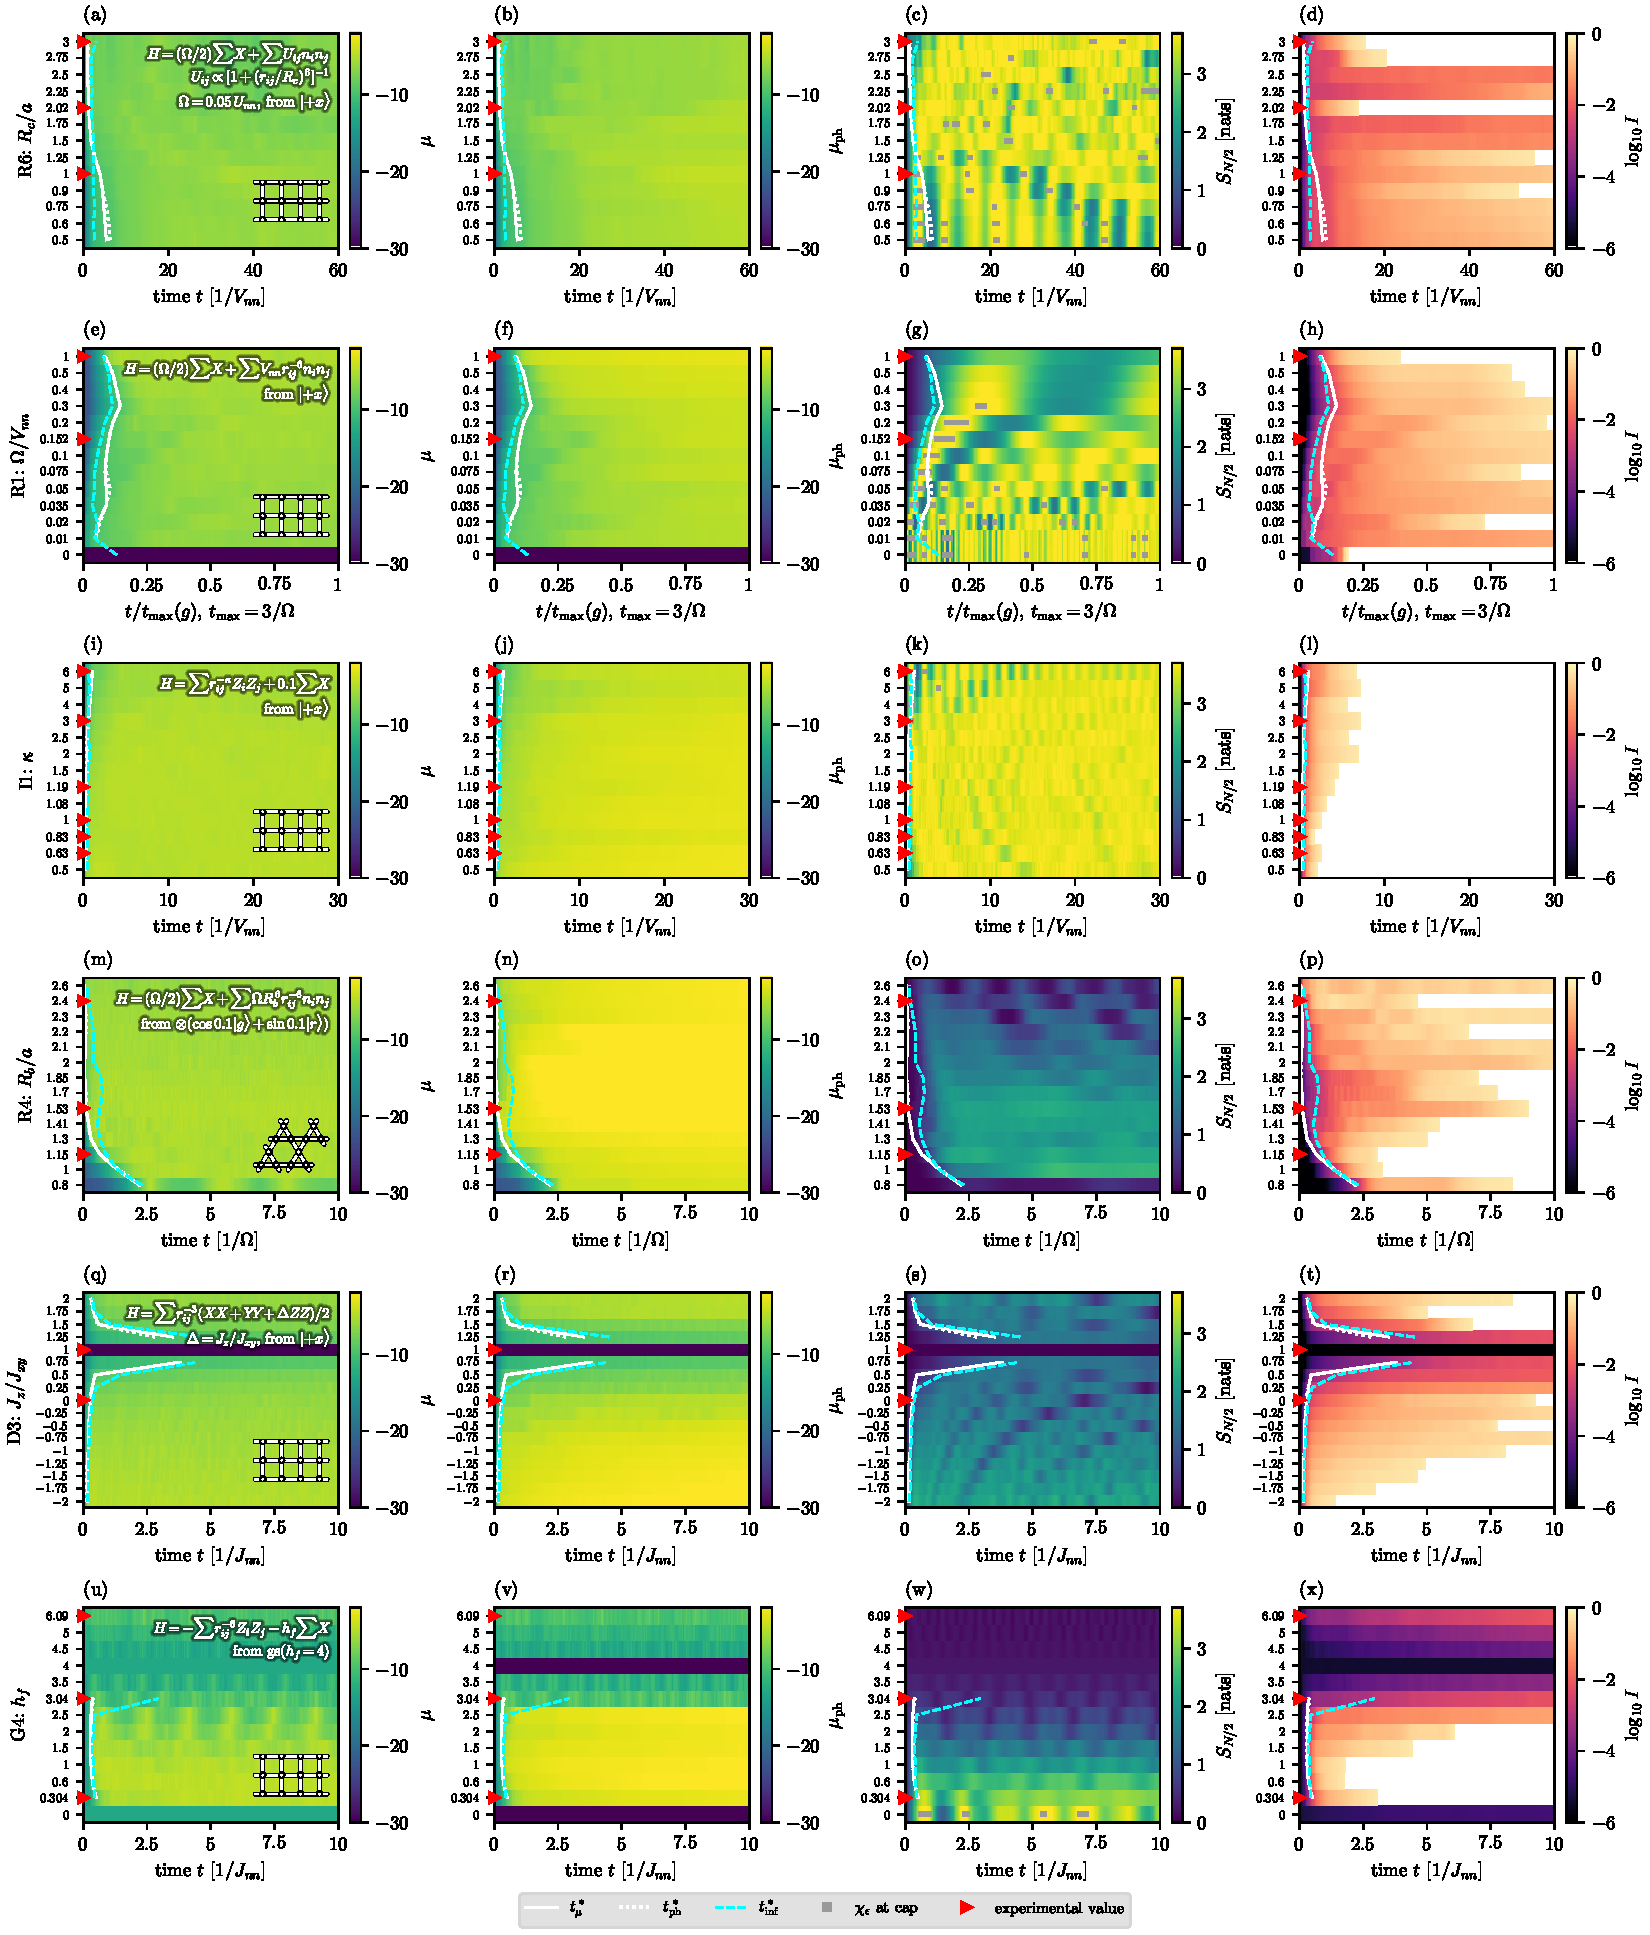
\includegraphics[width=\linewidth]{main_rows}
  \caption{As Fig.~\ref{fig:main-rows-hl}, for all six Stage-3 families.}
  \label{fig:main-rows}
\end{figure}

\begin{figure}[p]
  \centering
  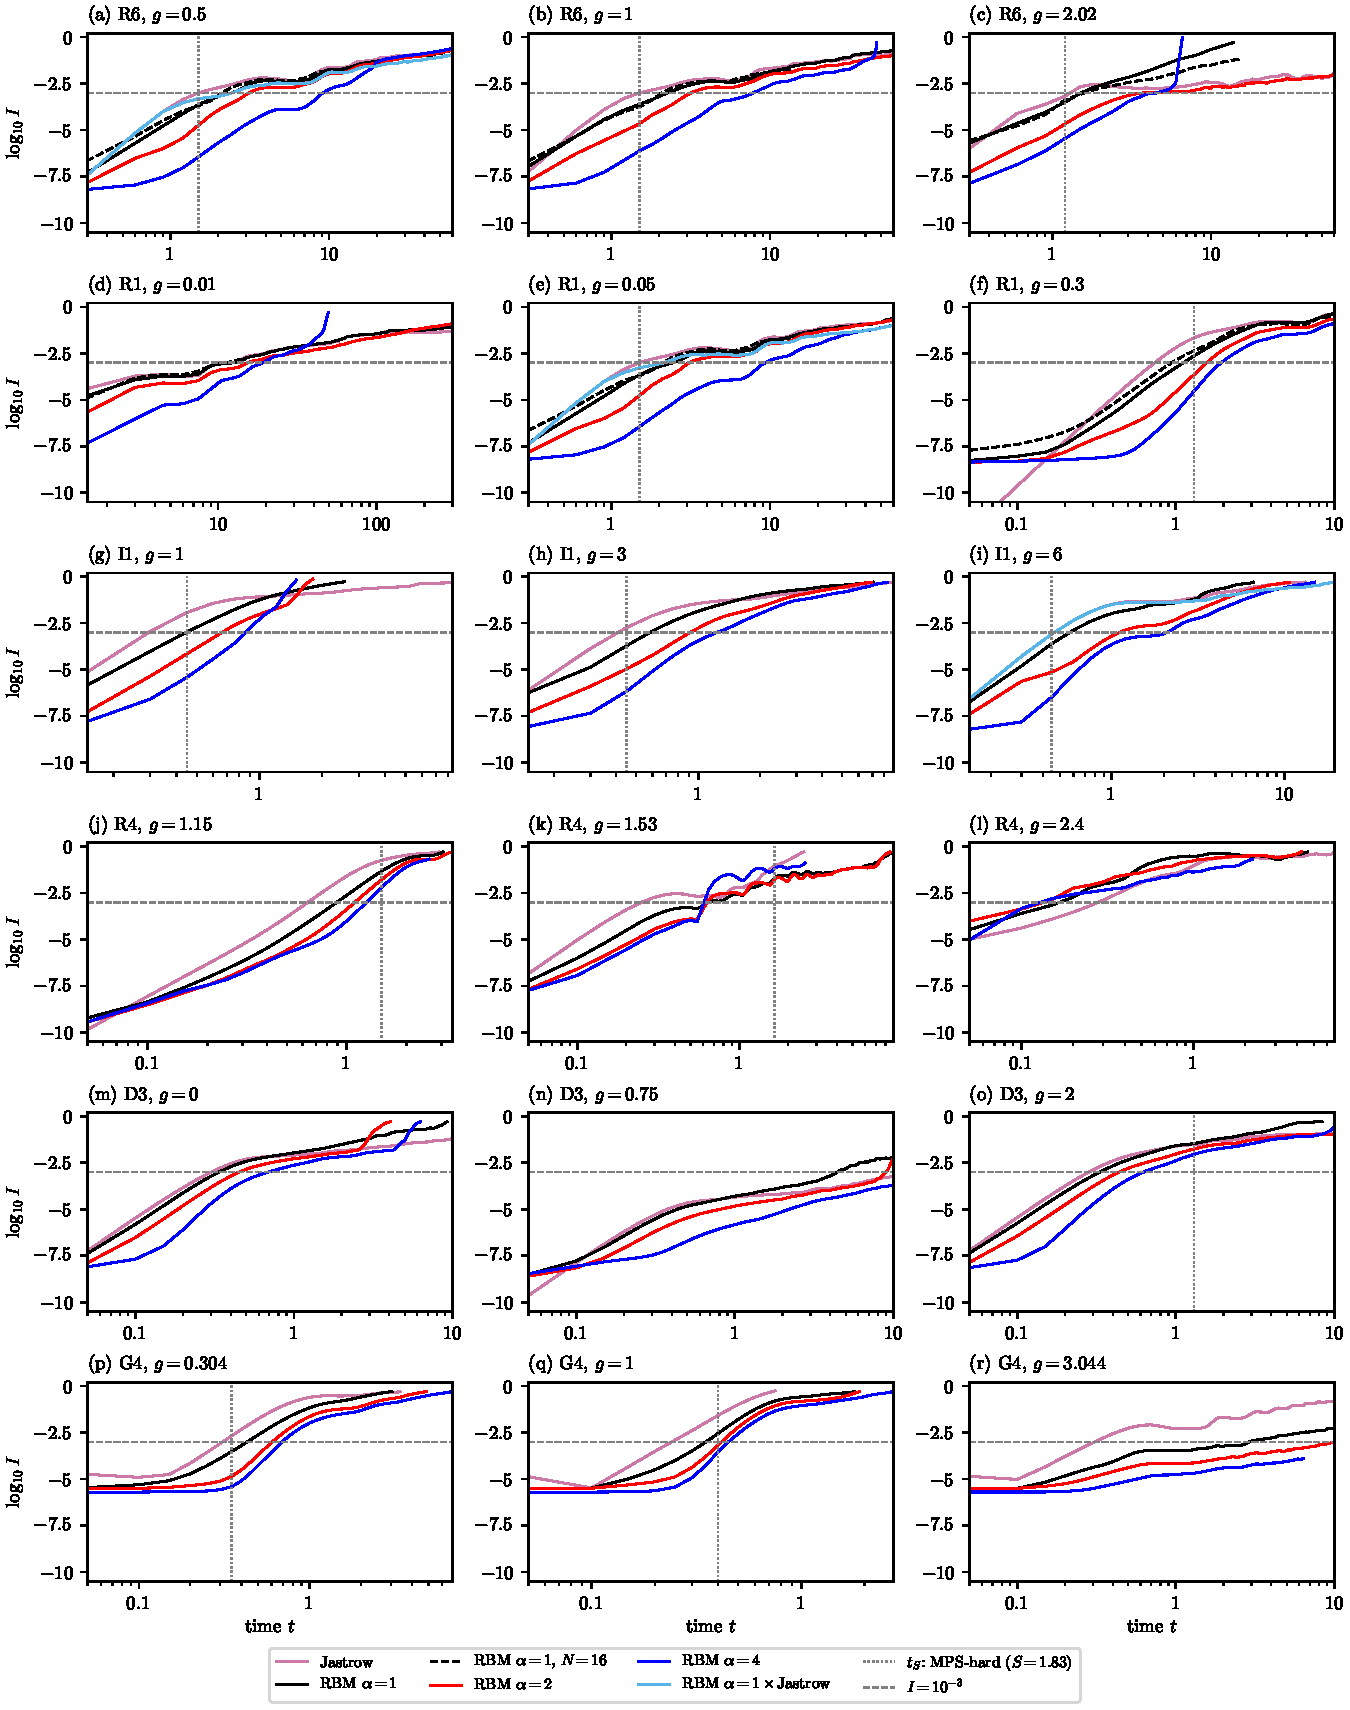
\includegraphics[width=\linewidth]{ansatz}
  \caption{As Fig.~\ref{fig:ansatz-hl}, for all six Stage-3 families. Times in the units of Fig.~\ref{fig:main-rows}.}
  \label{fig:ansatz}
\end{figure}

\begin{figure}[t]
  \centering
  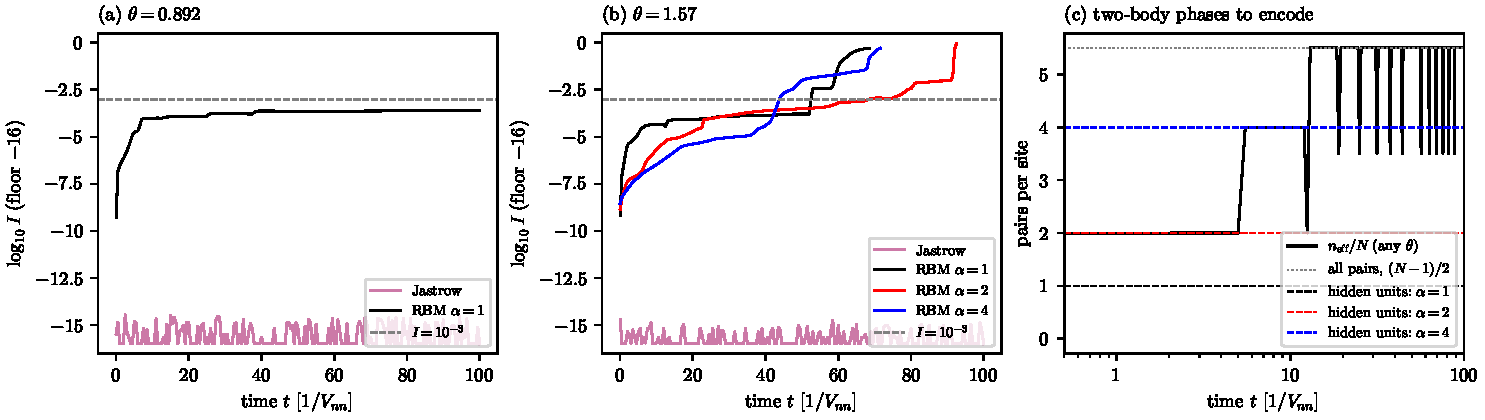
\includegraphics[width=\linewidth]{omega0}
  \caption{Representability at $\Omega=0$ (R0, kagome, $|\theta\rangle$ start). (a,b)~$\log_{10}\inff(t)$ per ansatz
    at $\theta=0.892$ and $\pi/2$; the Jastrow factor is exact to machine precision. (c)~Number of non-trivial pair
    phases per site, $n_{\mathrm{eff}}/N$, against the hidden-unit densities $\alpha$.}
  \label{fig:omega0}
\end{figure}

\begin{figure}[t]
  \centering
  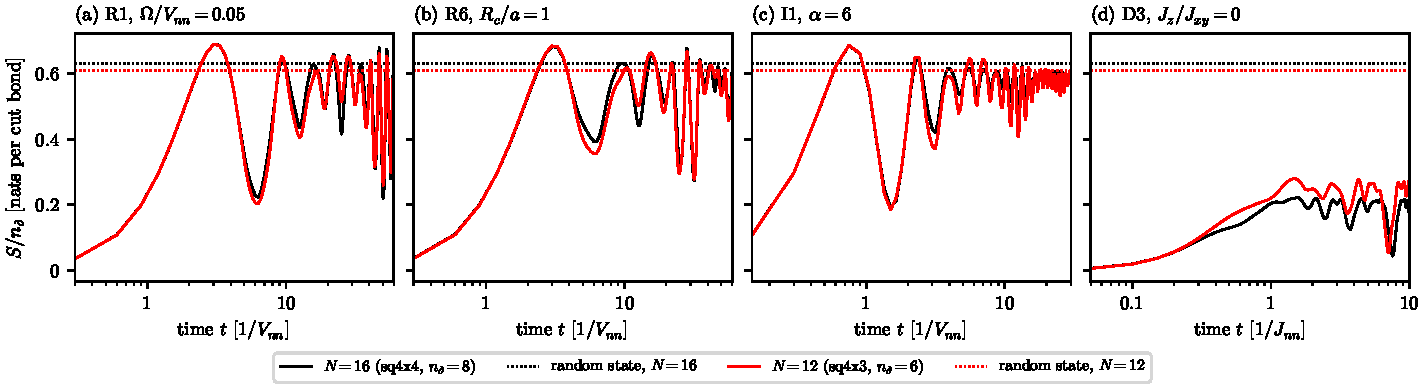
\includegraphics[width=0.8\linewidth]{scaling}
  \caption{Half-cut entropy per cut boundary bond, $S/n_\partial$, for $N=12$ (\texttt{sq4x3}, black) and $N=16$
    (\texttt{sq4x4}, red) at four near-classical points; dotted: Page values per bond.}
  \label{fig:scaling}
\end{figure}

\paragraph{Results for the other families.}
\begin{itemize}
  \item \emph{R6} behaves like R1 ($t_S=1.2$--$1.5$; $\inff<10^{-3}$ up to $t=1.5$--$2.7$ with $\alpha=1$ over the
    whole grid, $3.0$--$3.6$ with $\alpha=2$, $4.5$--$9.0$ with $\alpha=4$). At the experimental
    $R_c/a=2.02$~\cite{Zeiher16} the RBM window is $1.5$ ($\alpha=1$) to $4.5$ ($\alpha=4$). Jastrow alone: $\tinf=1.5$
    vs $2.7$ ($R_c/a=0.5$); RBM$\times$Jastrow: $2.7$ vs $2.7$. $\alpha=4$ is not uniformly better: at $2.02$ it
    becomes unstable at $t\approx5$ (Fig.~\ref{fig:ansatz}c). At $N=16$: $\tinf$ $2.7\to2.4$ ($0.5$), $2.4\to2.1$
    ($1.0$), $1.8\to1.8$ ($2.02$).
  \item \emph{D3, R4 (non-classical).} The $\alpha=1$ RBM crosses $10^{-3}$ at $t=0.15$--$1.5$, except near special
    points (D3 around $J_z/J_{xy}=1$, where $|{+}x\rangle$ is an eigenstate). At the hard points larger $\alpha$ shifts
    $\tinf$ by at most $\approx2\times$. R4 is hard for all ansätze from $t\approx0.2$--$1$ even where $\eta\le0.01$
    ($R_b/a\ge2$); the cause was not established.
  \item \emph{I1 is near-classical ($\eta\le0.08$) but fails at $t_S$.} The $\alpha=1$ RBM crosses $10^{-3}$ at
    $t=0.45$--$0.75$, just at or after $t_S=0.45$; $\alpha=4$ extends this to $0.9$--$2.1$; RBM$\times$Jastrow at
    $\kappa=6$: $0.6$ vs $0.6$. The long-range Ising phases ($r^{-\kappa}$ couplings to all sites) build up within
    $t\lesssim1$, much faster than in R1/R6.
  \item \emph{$\Omega=0$ (R0, Fig.~\ref{fig:omega0}).} Let $n_{\mathrm{eff}}=\#\{i<j:\ |\sin2c^{\mathrm{ph}}_{ij}|>0.1\}$,
    with $c^{\mathrm{ph}}_{ij}$ the two-body coefficients of the phase: the number of pair phases that are not
    multiples of $\pi/2$, i.e.\ the number of two-body gates an RBM has to encode. The exact Jastrow state stays at
    $\inff\sim10^{-16}$ for $t\le100$. The RBMs, which can represent it in principle, drift: at $\theta=\pi/2$,
    $\tinf=52$ ($\alpha=1$), $68$ ($\alpha=2$) and $44$ ($\alpha=4$); at $\theta=0.892$ the $\alpha=1$ RBM stays at
    $\inff\approx3\times10^{-4}$ up to $t=100$. Since $n_{\mathrm{eff}}/N$ reaches $5.5$ (all pairs) by $t\approx13$,
    $\alpha\gtrsim n_{\mathrm{eff}}/N$ is neither necessary (at $\theta=0.892$, $\alpha=1$ suffices) nor sufficient
    (at $\pi/2$, $\alpha=4$ fails first): the limitation at $\Omega=0$ is the TDVP integration, not the expressivity.
  \item \emph{S3 (Clifford kicked Ising).} $\mu_{\mathrm{ph}}$ is above $-10$ from the first save (see the screen
    results above), and the $\alpha=1$ RBM reaches $\inff=0.95$--$0.99$ after one save step. Stabilizer states have
    exact RBM representations~\cite{Deng17}, so this is a failure of TDVP on the kicked protocol, whose cause we did
    not investigate.
  \item \emph{I5}, the screen's best non-classical window, gives no RBM information: the RBM does not move. Its
    infidelity equals $1-|\langle\psi_0|\psi_{\mathrm{ED}}(t)\rangle|^2$ to three digits ($0.067$ at $t=0.05$) for
    both $\alpha=1$ and $2$. With zero hidden biases $\log\cosh$ is even in $s$, so at initialisation the TDVP
    tangent space contains no odd three-body term $Z_iZ_jZ_k$. Random hidden biases would be needed to test I5 (not
    done).
\end{itemize}

\paragraph{Proxy validity, all families} (Tables~\ref{tab:rydcorr}, \ref{tab:rydorder}).
\begin{itemize}
  \item $\mu_{\mathrm{ph}}$ is the best single predictor in D3, G4, R1 and I1 ($\rho=0.82$--$0.94$; after
    controlling for $S$: $0.80$--$0.93$). $\mu$ is close behind; $S$ adds little once $\mu$ is known
    ($\rho(S|\mu)\le0.19$ in all six families), and neither does the $\chi_\varepsilon$ fraction.
  \item R6 is weaker ($0.79/0.75$, dropping to $0.62/0.39$ after also controlling for $t$), and R4 fails
    ($\rho(\mu)=0.10$): its infidelity rises within $t\lesssim1$ for every $R_b/a$, while $\mu$ varies little.
  \item $\tprox$ orders $\tinf$ across $g$ with $\rho=0.97$ (D3), $1.00$ (R1), $0.72$--$0.73$ (R4), $0.64$--$0.72$
    (G4) and $0.56$--$0.59$ (R6, I1). In the non-classical families (D3, G4, R4) the proxies fire first
    ($\tinf/\tprox\approx1.3$--$3.5$); in the near-classical ones they fire late (R1 at all 12 points, R6 at 6 of 13).
  \item \emph{MPS-hard / NQS-easy quadrant} ($\chi_\varepsilon$ at $\ge90\%$ of its cap and $\inff<10^{-3}$): 343 of
    20356 points. Apart from the exactly classical points (R0, R1 at $\Omega=0$, G4 at $h_f=0$) they belong to R1
    ($\Omega/V_{nn}\le0.3$, $t\le9$), R6 ($t\le9$), I1 ($t\le1.05$) and G4 at $h_f=0.304$ ($t\le0.65$). The largest
    $\eta$ in the quadrant is $0.23$.
\end{itemize}

\begin{table}[h]
  \centering
  \caption{Spearman correlation $\rho$ of each proxy with $\log_{10}\inff$ ($\alpha=1$, $N=12$, all $g$ and
    $t>0$), and partial correlations controlling for $S$, for $(S,t)$, and for $\mu$. $n$: number of $(g,t)$ points.}
  \label{tab:rydcorr}
  \footnotesize
  \setlength{\tabcolsep}{4pt}
  \begin{tabular}{lr@{\hspace{1.2em}}rrr@{\hspace{1.2em}}rr@{\hspace{1.2em}}rr@{\hspace{1.2em}}rr}
    \toprule
    & & \multicolumn{3}{c}{$\rho$} & \multicolumn{2}{c}{$\rho(\cdot|S)$} & \multicolumn{2}{c}{$\rho(\cdot|S,t)$}
      & \multicolumn{2}{c}{$\rho(\cdot|\mu)$}\\
    family & $n$ & $\mu$ & $\mu_{\mathrm{ph}}$ & $S$ & $\mu$ & $\mu_{\mathrm{ph}}$ & $\mu$ & $\mu_{\mathrm{ph}}$
      & $\mu_{\mathrm{ph}}$ & $S$\\
    \midrule
    R1 & 2430 & 0.85 & 0.92 & 0.14 & 0.86 & 0.92 & 0.85 & 0.91 & 0.65 & 0.19\\
    R6 & 2270 & 0.79 & 0.75 & 0.04 & 0.79 & 0.75 & 0.62 & 0.39 & 0.29 & 0.12\\
    I1 & 396  & 0.78 & 0.82 & 0.37 & 0.75 & 0.80 & 0.71 & 0.72 & 0.43 & 0.19\\
    R4 & 2000 & 0.10 & 0.38 & 0.17 & $-0.06$ & 0.36 & $-0.07$ & $-0.40$ & 0.40 & 0.15\\
    D3 & 2580 & 0.89 & 0.93 & 0.67 & 0.80 & 0.87 & 0.84 & 0.88 & 0.57 & 0.04\\
    G4 & 1941 & 0.91 & 0.94 & 0.29 & 0.90 & 0.93 & 0.92 & 0.95 & 0.59 & 0.04\\
    \midrule
    pooled & 11965 & 0.82 & 0.83 & 0.32 & 0.80 & 0.84 & 0.83 & 0.85 & 0.39 & 0.19\\
    \bottomrule
  \end{tabular}
\end{table}

\begin{table}[h]
  \centering
  \caption{Onset ordering across $g$ ($\alpha=1$, $N=12$). $\rho$: Spearman of $\tmu$ (resp.\ $\tph$) with $\tinf$
    over the grid points where both are finite ($n$); last two columns: median of $\tinf/\tprox$, and the
    fraction of points at which the RBM fails before either proxy fires.}
  \label{tab:rydorder}
  \small
  \begin{tabular}{lrrrrr}
    \toprule
    family & $n$ & $\rho(\tmu,\tinf)$ & $\rho(\tph,\tinf)$ & median $\tinf/\tprox$ & RBM first\\
    \midrule
    R1 & 12 & 1.00 & 1.00 & 0.77 & 100\%\\
    R6 & 13 & 0.56 & 0.56 & 1.33 & 46\%\\
    I1 & 13 & 0.59 & 0.59 & 1.50 & 23\%\\
    R4 & 14 & 0.72 & 0.73 & 3.50 & 0\%\\
    D3 & 16 & 0.97 & 0.97 & 1.29 & 0\%\\
    G4 & 8 & 0.64 & 0.72 & 1.33 & 13\%\\
    \bottomrule
  \end{tabular}
\end{table}

\begin{table}[h]
  \centering
  \caption{Closest candidates to a quantum RBM advantage ($N=12$). $t_S$: first time with $S_{\mathrm{rel}}\ge0.5$
    ($\infty$: never); $\tinf$ and $\inff(t_S)$ for the best ansatz tried.}
  \label{tab:gold}
  \scriptsize
  \setlength{\tabcolsep}{3pt}
  \begin{tabular}{lllrrrrrl}
    \toprule
    ID & $g$ & $\eta$ & $S_{\mathrm{rel}}^{\max}$ & $t_S$ & $\tmu$ / $\tph$ & best $\tinf$ & $\inff(t_S)$ & why it fails\\
    \midrule
    S3 & $h=0$ & 0.61 & 1.14 & 2 & 2 / 2 & 2 & 0.99 & $\inff\approx1$ after one save step\\
    S3 & $h=\pi/4$ & 0.52 & 1.14 & 2 & 2 / 2 & 2 & 0.95 & same\\
    G4 & $h_f=1.0$ & 0.61 & 0.64 & 0.40 & 0.30 / 0.30 & 0.45 & $2.8\times10^{-4}$ & proxies fire before $t_S$\\
    D3 & $J_z/J_{xy}=2$ & 0.58 & 0.55 & 1.3 & 0.30 / 0.30 & 0.65 & $9\times10^{-3}$ & RBM fails before $t_S$\\
    D3 & $J_z/J_{xy}=0.75$ & 0.88 & 0.40 & $\infty$ & 3.75 / 3.85 & $>10$ & -- & never MPS-hard\\
    I5 & $h_x=0.5$ & 0.31 & 0.48 & $\infty$ & $\infty$ / $\infty$ & 0.05 & -- & never MPS-hard; RBM frozen\\
    G4 & $h_f=0.304$ & 0.23 & 0.95 & 0.35 & 0.50 / 0.50 & 0.70 & $3.9\times10^{-6}$ & $\eta<0.3$; proxy window $1.4$\\
    R1 & $\Omega=0.3$ & 0.15 & 1.06 & 1.3 & 1.45 / 1.45 & 1.95 & $3.0\times10^{-5}$ & $\eta<0.3$\\
    \bottomrule
  \end{tabular}
\end{table}

\FloatBarrier
\section{Numerical details}
\label{app:num}

\paragraph{Part I, TDVP.} Adaptive RK45 integrator with initial $dt=0.01$, a dense holomorphic QGT
(\texttt{QGTJacobianDense}) and NetKet's default linear solver, identical for every run.

\paragraph{Part II, exact evolution.} Sparse Pauli-string Hamiltonians, evolved with \texttt{expm\_multiply} from
\texttt{scipy.sparse.linalg}, with sub-steps $dt\le\min(\Delta t_{\mathrm{save}},\,0.1/\max_s\sum_{s'}|H^{\mathrm{off}}_{ss'}|)$.
Piecewise-constant protocols (kicked Ising, QAOA, and the modulated drive of family C2, 24 pieces per drive period) are
evolved segment by segment; diagonal segments exactly. The phase is unwrapped exactly for the diagonal part of each
sub-step and by continuity for the rest: $\varphi\leftarrow\varphi+\arg(\psi_{\mathrm{new}}\bar\psi_{\mathrm{old}}e^{iE_d\,dt})-E_d\,dt$.
Lattice sites map to bit $N-1-i$ of the basis index, with $s_i=+1\leftrightarrow|{\uparrow}\rangle$, as in NetKet.

\paragraph{Part II, TDVP.} NetKet~3.19 TDVP with adaptive RK45 ($dt_0=0.01$; $10^{-4}$ for R4, which otherwise fails
at $R_b/a=2.4$), dense holomorphic QGT, the QGT error norm, and a smooth pseudo-inverse with $r_{\mathrm{tol}}=10^{-8}$.
One TDVP driver per Floquet segment.

\paragraph{Software issues.} NetKet~3.19's adaptive RK step recompiles a \texttt{lax.cond} at every step (unbounded
memory); we patched it to run the branch eagerly, which leaves the step sequence unchanged. An early version of our
save loop matched NetKet's \texttt{iter} stops (which use \texttt{np.isclose}, rtol $10^{-5}$) to the exact save
times and silently stopped recording; all affected runs were repeated with an explicit integration to each save time.

\section{Reproducibility}
\sloppy
All code lives in \texttt{check\_time\_evolution/} and was run with the project \texttt{.venv} on CPU. Part~I code is in \texttt{quench2d/} and Part~II code in \texttt{rydberg/}. Each folder has its own \texttt{data/} and \texttt{figs/}. Run each script from its own folder; the paths below are relative to that folder.
\begin{itemize}
  \item \texttt{quench2d.py}: lattice, dense and NetKet Hamiltonians, ED evolution, WHT and
    Fermi--Dirac analysis. \texttt{A0\_FACTOR} switches $A_0$. Running
    \texttt{python quench2d.py} checks the FWHT, the SU(2) eigenstate, and that the NetKet and dense
    $H$ agree.
  \item \texttt{ed\_scan.py}: all ED scans and the 1D calibration, which write
    \texttt{data/ed\_*.npz}. The scans are the XY-coupling quench (code label B), the field quench (A), the plane,
    $dt/2$, and $h_0=6$.
  \item \texttt{rbm\_run.py FAM VAL ALPHA}: one RBM+TDVP run, which writes
    \texttt{data/rbm/rbm\_*.npz}. The batch is \texttt{data/rbm/run\_batch.sh} with the job list
    \texttt{data/rbm/jobs.txt}.
  \item \texttt{analysis.py}: writes \texttt{data/table\_long.csv}, \texttt{table\_tstar.csv},
    \texttt{table\_tstar\_plane.csv} and \texttt{correlations.csv}.
  \item \texttt{make\_figs.py}: writes every Part-I figure in \texttt{figs/}.
  \item \texttt{rydberg2d.py}: lattices, Rydberg/dipolar/Ising/circuit Hamiltonians, sparse evolution with phase
    unwrapping (\texttt{python rydberg2d.py} runs the self-checks).
  \item \texttt{rydberg\_screen.py}: family specifications and the Stage-1 screen, writing
    \texttt{data/screen/<ID>\_<lattice>\_<init>.npz}; \texttt{rydberg\_triage.py}: triage tables
    \texttt{data/triage*.csv}.
  \item \texttt{rydberg\_rbm.py ID LAT INIT G ANSATZ}: one RBM/Jastrow+TDVP run, writing
    \texttt{data/rbm/*.npz}; batch runner \texttt{data/run\_rbm\_jobs.sh} with job lists
    \texttt{data/*jobs*.txt}.
  \item \texttt{rydberg\_analysis.py}: \texttt{data/rbm\_long.csv}, \texttt{rbm\_tstar.csv},
    \texttt{rbm\_corr.csv}, \texttt{rbm\_order.csv}; \texttt{rydberg\_figs.py screen|map|scaling|main|omega0|ansatz}:
    the Part-II figures in \texttt{figs/} (\texttt{main} and \texttt{ansatz} also write the R1+G4 versions \texttt{*\_hl}).
  \item References: \texttt{report/refs.bib}; experimental parameters: \texttt{data/exp\_params.csv}.
\end{itemize}

\bibliographystyle{unsrt}
\bibliography{refs}
\end{document}

